%%%% CAPÍTULO 3 - METODOLOGIA

\chapter{Metodologia}
\label{cap:metodologia}

Este capítulo aborda as metodologias de modelagem e desenvolvimento utilizadas no trabalho.

\section{Escopo do sistema}
\label{sec:escopoDoSistema}

O sistema \textit{Virtual Lab} deve possibilidar a criação e gerenciamento de instâncias de máquinas virtuais para uso em laboratórios remotos de ensino e pesquisa.
O acesso deve ser feito por meio de um navegador de internet, permitindo a utilização de qualquer dispositivo com um navagador de internet com acesso à rede.

O sistema deve acomodar dois tipos de usuários: usuários comuns e administradores.
Os usuários comuns devem ter permissão de criar instâncias de máquinas virtuais com base em templates pré-definidos, gerenciar suas próprias instâncias, bem como o conteúdo instalado nas mesmas.
Os administradores devem ter as mesmas permissões dos usuários comuns, além de gerenciar os templates de instância, controlar o acesso dos usuários comuns ao sistema e aos recursos de hardware.

O sistema deve permitir o acesso aos usuários através de autenticação por meio de usuário e senha, bem como através de um provedor de identidade externo, caso o ambiente de uso do sistema já possua um provedor de identidade.

Inicialmente, um usuário administrador deve criar os templates de instância indicando o sistema operacional e a quantidade de armazenamento disponível.
Os usuários comuns devem então criar instâncias com base nesses templates, escolhendo entre os tipos de hardware permitidos.

Ao ser criada, a instância deve passar por um processo de configuração inicial para garantir que o sistema operacional esteja pronto para uso, e então ser disponibilizada para o usuário, que poderá acessá-la atráves da página de conexões do sistema. As instâncias devem ser encerradas automaticamente após um período de inatividade.

\section{Modelagem}
\label{sec:modelagemDoSistema}

O processo de modelagem do sistema partiu de alguns princípios elementares para a construção de um sistema de software: 

\begin{itemize}
    \item \textbf{Objetividade}: Criar apenas modelos que sejam necessários para a compreensão do sistema. Modelos em excesso tornam o processo de desenvolvimento mais complexo e custoso.

    \item \textbf{Facilidade de alteração}: Os modelos devem ser fáceis de serem alterados, de forma que as mudanças no sistema possam ser refletidas rapidamente nos modelos. Esse princípio é de extrema importância tanto para a extensibilidade do sistema quanto para o isolamento dos componentes em cenários de teste.

    \item \textbf{Arquitetura do sistema em primeiro lugar}: Na concepção dos componentes do sistema, é importante considerar a arquitetura do sistema como um todo, de forma que os componentes sejam coesos e acoplados de forma apropriada. Esse princípio também é relevante quando pensamos na utilização de serviços de computação em nuvem, que possuem características próprias de arquitetura, infraestrutura, segurança e modelo de cobrança.

    \item \textbf{Componentes funcionalmente independentes}: Os componentes do sistema devem ser independentes entre si, isso não significa que eles não possam se comunicar, mas que o nível de encapsulamento deve entregar funcionalidades claras e bem definidas.

    \item \textbf{Consistência das informações em todos os níveis}: As informações que são transmitidas entre os componentes do sistema devem ser verificadas e validadas em todos os níveis, garantindo que a integridade do sistema seja mantida.

\end{itemize}

O processo de modelagem do sistema foi dividido nas seguintes etapas: levantamento de requisitos, projeto de arquitetura e projeto de componentes \citep{pressman2016}.

\subsection{Levantamento de Requisitos}
\label{subsec:levantamentoDeRequisitos}

% especificação dos requisitos funcionais e não funcionais, e casos de uso

Inicialmente, os requisitos do sistema foram identificados a partir de discussões recorrentes com o orientador do trabalho, que possui experiência em desenvolvimento de sistemas de software e em ambientes de ensino e pesquisa. Além disso, é um dos responsáveis pelo gerenciamento dos recursos de infraestrutura da \gls{utfpr} servidos em nuvem publica através da \gls{aws}.

Os requisitos foram divididos em funcionais e não funcionais, e como uma forma de orientar o desenvolvimento, foram criados casos de uso para representar as interações entre os usuários e o sistema.

As Tabelas \ref{tab:requisitosFuncionaisDoSistema} e \ref{tab:requisitosNaoFuncionaisDoSistema} apresentam os requisitos funcionais e não funcionais do sistema, respectivamente.

\begin{longtable}{@{\extracolsep{\fill}}l p{.8\textwidth}}%% Ambiente longtable
\caption{Requisitos funcionais do sistema\label{tab:requisitosFuncionaisDoSistema}} \\%% Legenda e rótulo
\toprule
\textbf{Identificador} & \textbf{Descrição} \\
\midrule
\endfirsthead%% Encerra cabeçalho da primeira página
\caption[]{Requisitos funcionais do sistema} \\%% Legenda
\multicolumn{2}{r}{\textbf{(continuação)}} \\
\toprule
\textbf{Identificador} & \textbf{Descrição} \\
% \midrule
\endhead%% Encerra cabeçalho das demais páginas
% \midrule
\multicolumn{2}{r}{\textbf{(continua)}} \\
\endfoot%% Encerra rodapé das demais páginas
% \bottomrule
\\[-0.5\linha]
\caption*{\nomefonte: Autoria própria (2024)} \\
\endlastfoot%% Encerra rodapé da última página

RF01 & Deve haver três tipos de permissões de usuário no sistema: \gls{upen}, \gls{ucom} e \gls{uadm} \\ \hline

RF02 & O usuário deve ser capaz de registrar-se no sistema utilizando um e-mail válido, senha e nome de usuário \\ \hline

RF03 & O usuário deve ser capaz de autenticar-se no sistema utilizando um e-mail válido e senha \\ \hline

RF04 & O usuário deve ser capaz de autenticar-se no sistema utilizando um provedor de identidade externo \\ \hline

RF05 & O usuário deve ser capaz de encerrar a sessão no sistema \\ \hline

RF06 & O usuário deve ser capaz de confirmar seu endereço de e-mail \\ \hline

RF07 & O usuário deve ser capaz de ver suas informações de perfil \\ \hline

RF08 & O usuário deve ser capaz de visualizar as suas cotas de uso no sistema \\ \hline

RF09 & Tanto o \gls{ucom} quanto o \gls{uadm} devem ser capazes de criar instâncias com base em templates de instância e suas cotas de uso disponíveis \\ \hline

RF10 & Tanto o \gls{ucom} quanto o \gls{uadm} devem ser capazes de listar de forma paginada as instâncias que possuem \\ \hline

RF11 & Tanto o \gls{ucom} quanto o \gls{uadm} devem ser capazes de visualizar detalhes, como estado e recursos, das instâncias que possuem \\ \hline

RF12 & Tanto o \gls{ucom} quanto o \gls{uadm} devem ser capazes de excluir instâncias que possuem \\ \hline

RF13 & Tanto o \gls{ucom} quanto o \gls{uadm} devem ser capazes de ligar instâncias desligadas que possuem \\ \hline

RF14 & Tanto o \gls{ucom} quanto o \gls{uadm} devem ser capazes de desligar instâncias ligadas que possuem \\ \hline

RF15 & Tanto o \gls{ucom} quanto o \gls{uadm} devem ser capazes de reiniciar instâncias ligadas que possuem \\ \hline

RF16 & Tanto o \gls{ucom} quanto o \gls{uadm} devem ser capazes de acessar as instâncias ligadas que possuem \\ \hline

RF17 & O \gls{uadm} deve ser capaz de listar de forma paginada todos os templates de instância disponíveis \\ \hline

RF18 & O \gls{uadm} deve ser capaz de criar templates de instância \\ \hline

RF19 & O \gls{uadm} deve ser capaz de editar templates de instância \\ \hline

RF20 & O \gls{uadm} deve ser capaz de excluir templates de instância \\ \hline

RF21 & O \gls{uadm} deve ser capaz de criar templates de instância a partir de suas instâncias \\ \hline

RF22 & O \gls{uadm} deve ser capaz de listar de forma paginada todos os usuários do sistema \\ \hline

RF23 & O \gls{uadm} deve ser capaz de editar a permissão de usuários do sistema \\ \hline

RF24 & O \gls{uadm} deve ser capaz de alterar a cota de uso de usuários do sistema \\ \hline

RF25 & O usuário deve ser capaz de visualizar as notificações enviadas pelo sistema \\ \hline

RF26 & O sistema deve ser capaz de enviar notificações para os usuários alertando sobre a mudança de estado de suas instâncias \\ \hline

RF27 & O sistema permitir o uso de filtros pré-definidos e busca textual para todos os recursos de listagem \\ 

RF28 & O sistema deve ser capaz de desligar automaticamente instâncias ociosas \\ \hline

RF29 & O sistema deve forcener uma lista de imagens de sistema operacional recomendadas para a criação de templates de instância \\ \hline

RF30 & O usuário deve ser capaz de acessar a documentação do sistema \\ \hline

\end{longtable}

\begin{longtable}{@{\extracolsep{\fill}}l p{.8\textwidth}}%% Ambiente longtable
\caption{Requisitos não funcionais do sistema\label{tab:requisitosNaoFuncionaisDoSistema}} \\%% Legenda e rótulo
\toprule
\textbf{Identificador} & \textbf{Descrição} \\
\midrule
\endfirsthead%% Encerra cabeçalho da primeira página
\caption[]{Requisitos não funcionais do sistema} \\%% Legenda
\multicolumn{2}{r}{\textbf{(continuação)}} \\
\toprule
\textbf{Identificador} & \textbf{Descrição} \\
% \midrule
\endhead%% Encerra cabeçalho das demais páginas
% \midrule
\multicolumn{2}{r}{\textbf{(continua)}} \\
\endfoot%% Encerra rodapé das demais páginas
% \bottomrule
\\[-0.5\linha]
\caption*{\nomefonte: Autoria própria (2024)} \\
\endlastfoot%% Encerra rodapé da última página

RNF01 & O sistema deve ser responsivo e acessível em dispositivos móveis, mesmo que algumas funcionalidades sejam limitadas \\ \hline

RNF02 & O sistema deve ser capaz de lidar com um grande número de usuários simultâneos \\ \hline

RNF03 & O sistema deve ser capaz de lidar com um grande número de instâncias simultâneas \\ \hline

RNF04 & O sistema deve atualizar as informações do estado das instâncias em tempo real, sem técnicas de \textit{polling}\footnote{O \textit{polling} é uma técnica utilizada para acompanhar o status de uma operação baseada na execução de requisições espaçadas por um intervalo de tempo pré-definido. Essa técnica pode ser custosa e esgotar os recursos do sistema}. \\ \hline

RNF05 & O sistema deve ser capaz de lidar com a criação de instâncias em menos de 5 minutos \\ \hline

RNF06 & O sistema deve apresentar eventuais erros de forma clara e objetiva \\ \hline

RNF07 & O sistema deve sinalizar ao usuário enquanto realiza operações assíncronas \\ \hline

RNF08 & O sistema deve tratar uma conexão como ativa com uma instância se a mesma estiver sendo feita a partir do sistema. Caso contrário, a instância será considerada ociosa \\ \hline

RNF09 & A documentação do sistema deve ser clara e objetiva, contendo explicações tanto sobre o funcionamento do sistema quanto sobre a utilização do sistema, além de apresentar todos os \textit{endpoints} da API \\ \hline

\end{longtable}


Os casos de uso do sistema foram modelados a partir dos requisitos funcionais identificados. De forma a dividir as responsabilidades do sistema em módulos, os casos de uso foram agrupados em quatro módulos principais: instância, template de instância, usuário e diversos, representados nas Figuras \ref{fig:casoDeUsoInstancia}, \ref{fig:casoDeUsoTemplate}, \ref{fig:casoDeUsoUsuario} e \ref{fig:casoDeUsoDiversos}, respectivamente.

Como pode ser visto no diagrama da \autoref{fig:casoDeUsoInstancia}, o módulo de instância necessitou de quatro interfaces para contextos distintos: Para usuários, para o sistema de provisionamento, para o sistema de envio de eventos das instâncias e para o gateway de conexão.

\begin{figure}[H]
%\captionsetup{width=0.55\textwidth}%% Largura da legenda
\caption{Diagrama de Caso de Uso: Instância}
\label{fig:casoDeUsoInstancia}
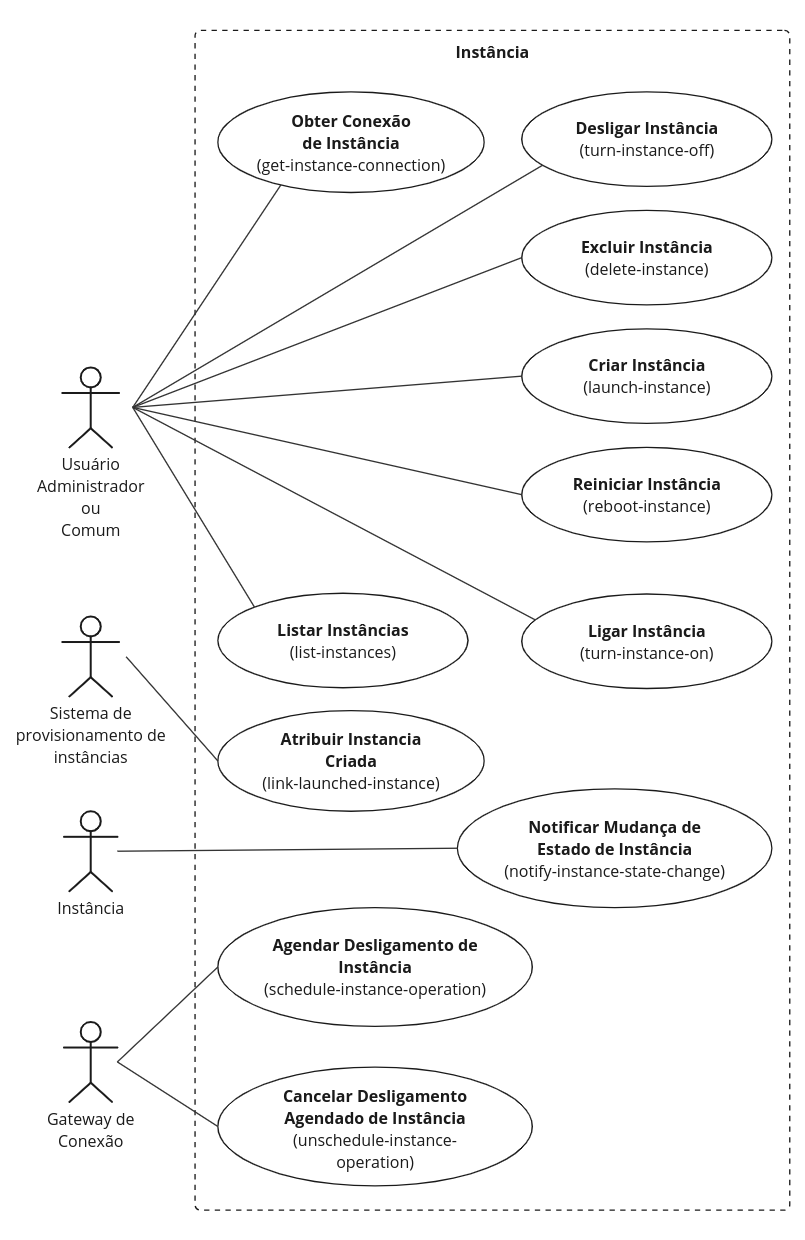
\includegraphics[width=\textwidth]{capitulos/2-metodologia/files/use-case-instance.png}
\fonte{Autoria Própria (2024)}
\end{figure}

O diagrama da \autoref{fig:casoDeUsoTemplate} apresenta o módulo de template de instância, que é essencial para a criação de instâncias no sistema, isso porque as instâncias são criadas a partir de templates que definem o sistema operacional e a quantidade de armazenamento disponível. Tanto o \gls{ucom} quanto o \gls{uadm} podem interagir com esse módulo, porém apenas o \gls{uadm} pode gerenciar os templates e criá-los a partir de instâncias existentes, está que é uma funcionalidade importante para a disponibilização de configurações personalizadas para diferentes cenários de aplicação do sistema.

\begin{figure}[H]
%\captionsetup{width=0.55\textwidth}%% Largura da legenda
\caption{Diagrama de Caso de Uso: Template de Instância}
\label{fig:casoDeUsoTemplate}
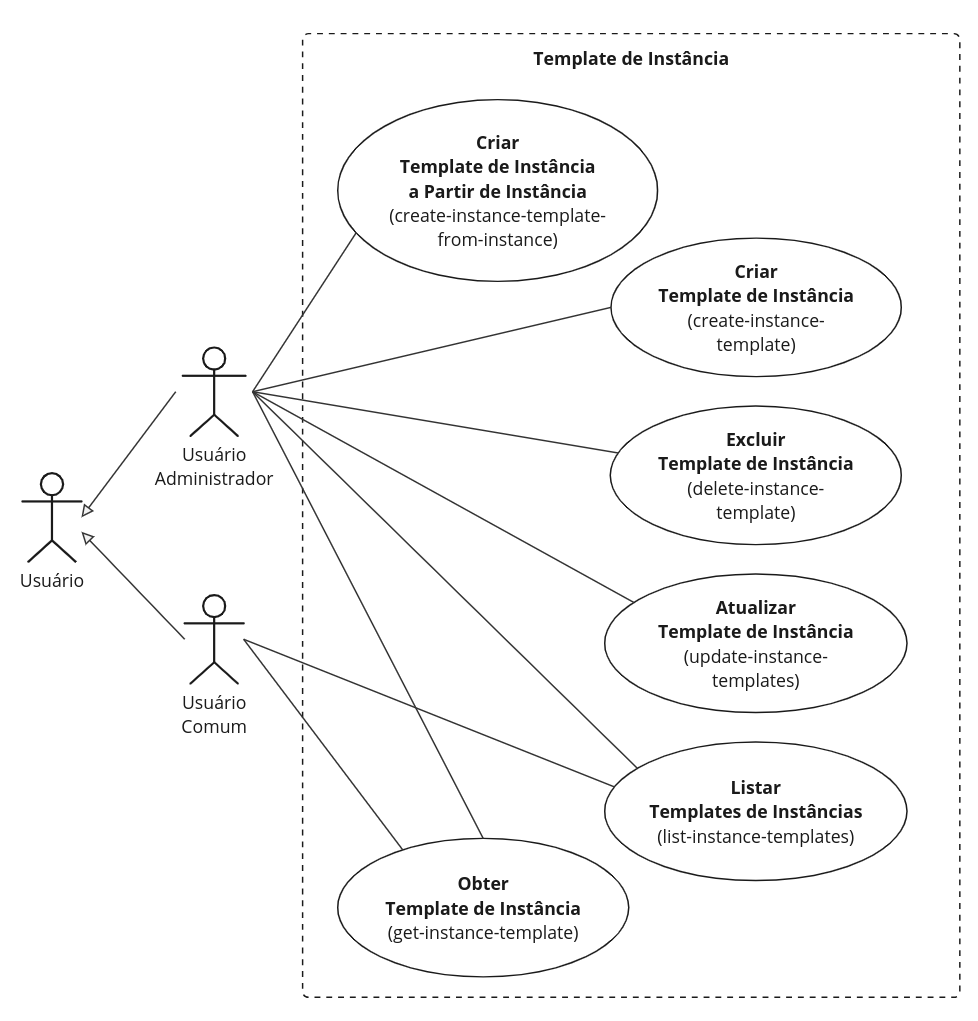
\includegraphics[width=\textwidth]{capitulos/2-metodologia/files/use-case-instance-template.png}
\fonte{Autoria Própria (2024)}
\end{figure}

No diagrama da \autoref{fig:casoDeUsoUsuario}, é possível notar que o atores que representam o usuário final do sistema não tem acesso aos casos de uso de criação de conta nem de de início de sessão. Isso porque o acesso ao sistema foi modelado para ser gerenciado por um serviço fora do contexto da implementação do sistema. Nesse caso, o sistema recebe os dados dos usuários através de gatilhos e então executa as operações para lidar apenas com dados não sensíveis e puramente operacionais.

\begin{figure}[H]
%\captionsetup{width=0.55\textwidth}%% Largura da legenda
\caption{Diagrama de Caso de Uso: Usuário}
\label{fig:casoDeUsoUsuario}
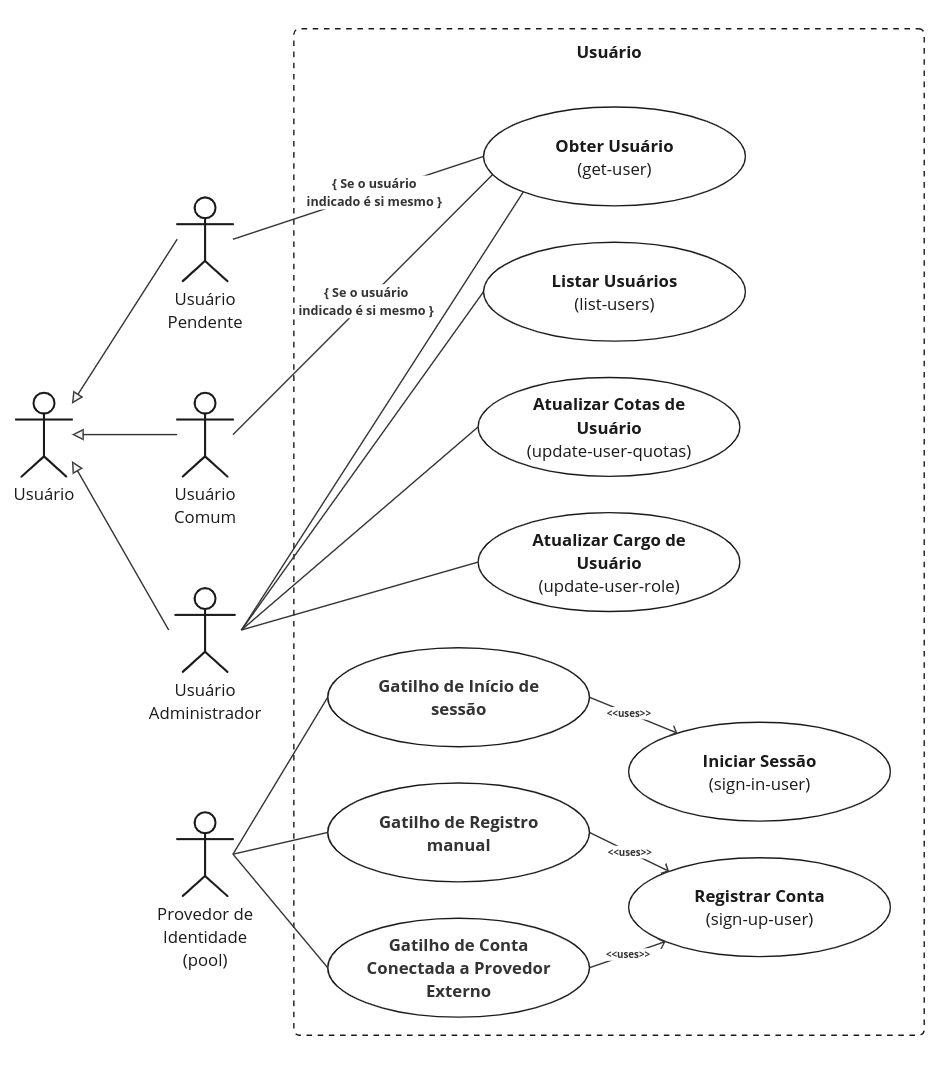
\includegraphics[width=\textwidth]{capitulos/2-metodologia/files/use-case-user.png}
\fonte{Autoria Própria (2024)}
\end{figure}

No caso do diagrama da \autoref{fig:casoDeUsoDiversos}, são apresentados apenas dois casos de uso auxiliares que servem para manter a consistência do sistema, permitindo que tanto a lista de tipos de instância quanto a lista de imagens de sistema operacional recomendadas sejam sugeridas de forma dinâmica, evitando assim a necessidade de sair do sistema para buscar informações ou até mesmo que o usuário tenha que memorizar informações que não são de seu interesse direto.

\begin{figure}[H]
%\captionsetup{width=0.55\textwidth}%% Largura da legenda
\caption{Diagrama de Caso de Uso: Diversos}
\label{fig:casoDeUsoDiversos}
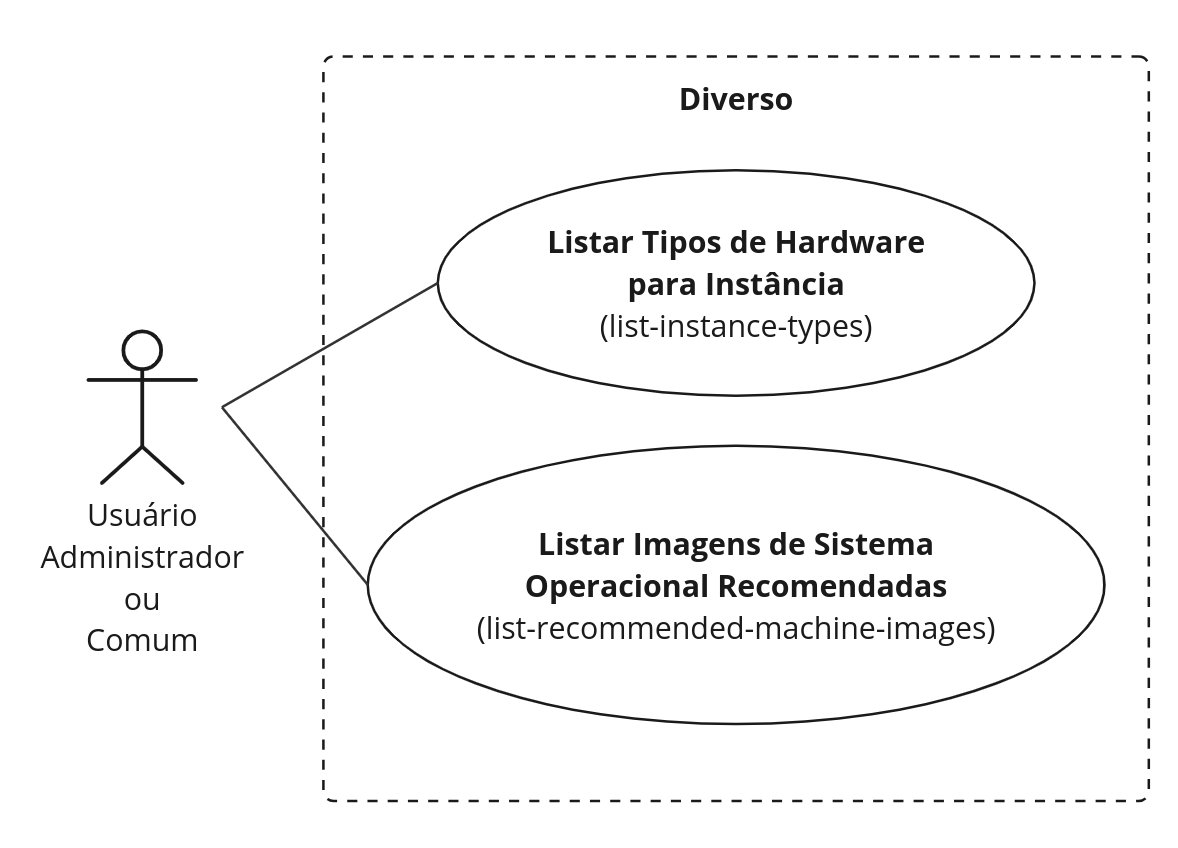
\includegraphics[width=\textwidth]{capitulos/2-metodologia/files/use-case-misc.png}
\fonte{Autoria Própria (2024)}
\end{figure}

\subsection{Projeto de Arquitetura}
\label{subsec:projetoDeArquitetura}
% Organização dos componentes.

Em seguida, o projeto de arquitetura do sistema foi elaborado a fim de produzir representações de alto nível dos componentes do sistema e das camadas de dado e serviço \citep{pressman2016}.

A apresentação do projeto de arquitetura foi construída utilizando o modelo de visualização de arquitetura de sistemas \textit{C4}, que promove uma abordagem partindo de uma visão abstrata até do sistema, passando por visões de contexto, \textit{containers} e componentes, de forma a facilitar a compreensão do sistema como um todo \citep{brown2018}.

A figura \autoref{fig:diagramaC4ContextoDoSistema} apresenta o diagrama de contexto do sistema, que mostra as interações do sistema com os atores externos, como os usuários e o provedor de identidade externo. Esse diagrama é a ponto de partida inicial para uma visão geral do contexto, onde o sistema em si é representado como um bloco central.

\begin{figure}[H]
%\captionsetup{width=0.55\textwidth}%% Largura da legenda
\caption{Diagrama C4: Contexto do Sistema}
\label{fig:diagramaC4ContextoDoSistema}
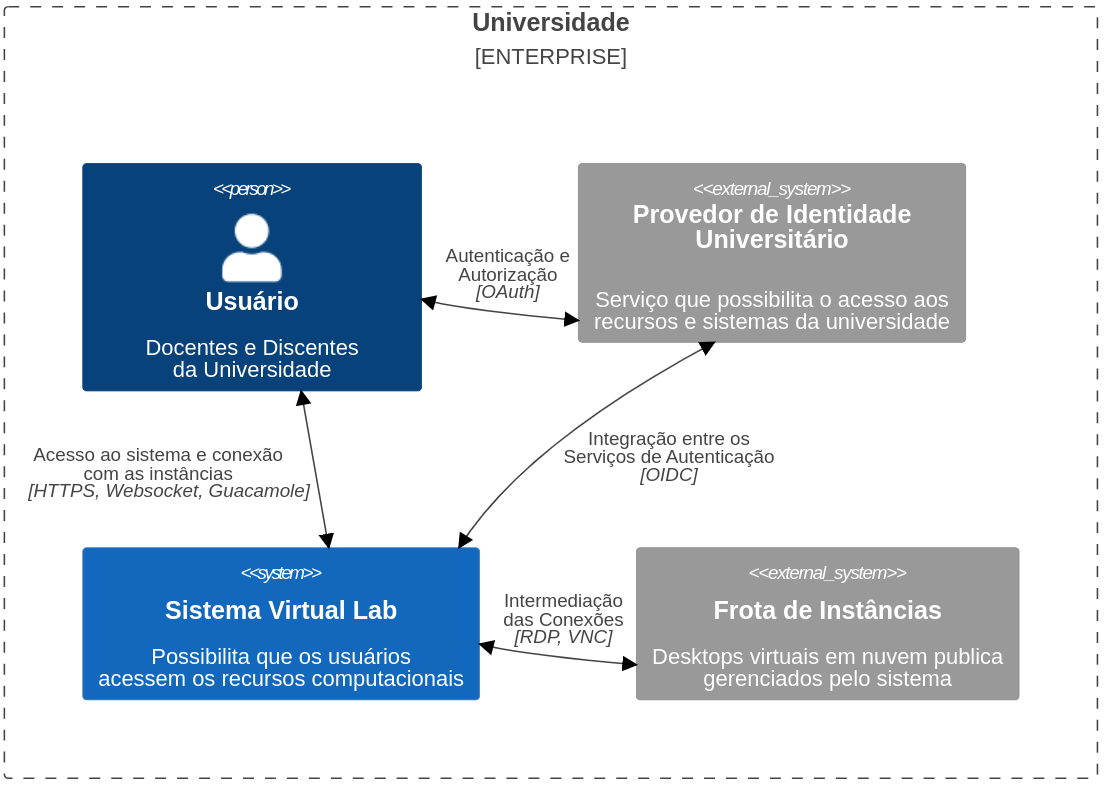
\includegraphics[width=\textwidth]{capitulos/2-metodologia/files/c4-system-context.png}
\fonte{Autoria Própria (2024)}
\end{figure}

Com uma ideia bem definida de como o sistema interage com o ambiente externo, o próximo passo foi a definição dos \textit{containers}, que são os componentes de alto nível que compõem o sistema, além de explicitar os protocolos de comunicação. O diagrama da \autoref{fig:diagramaC4ConteineresDoSistema} representa o resultado dessa etapa.

\begin{figure}[H]
%\captionsetup{width=0.55\textwidth}%% Largura da legenda
\caption{Diagrama C4: \textit{containers} do Sistema}
\label{fig:diagramaC4ConteineresDoSistema}
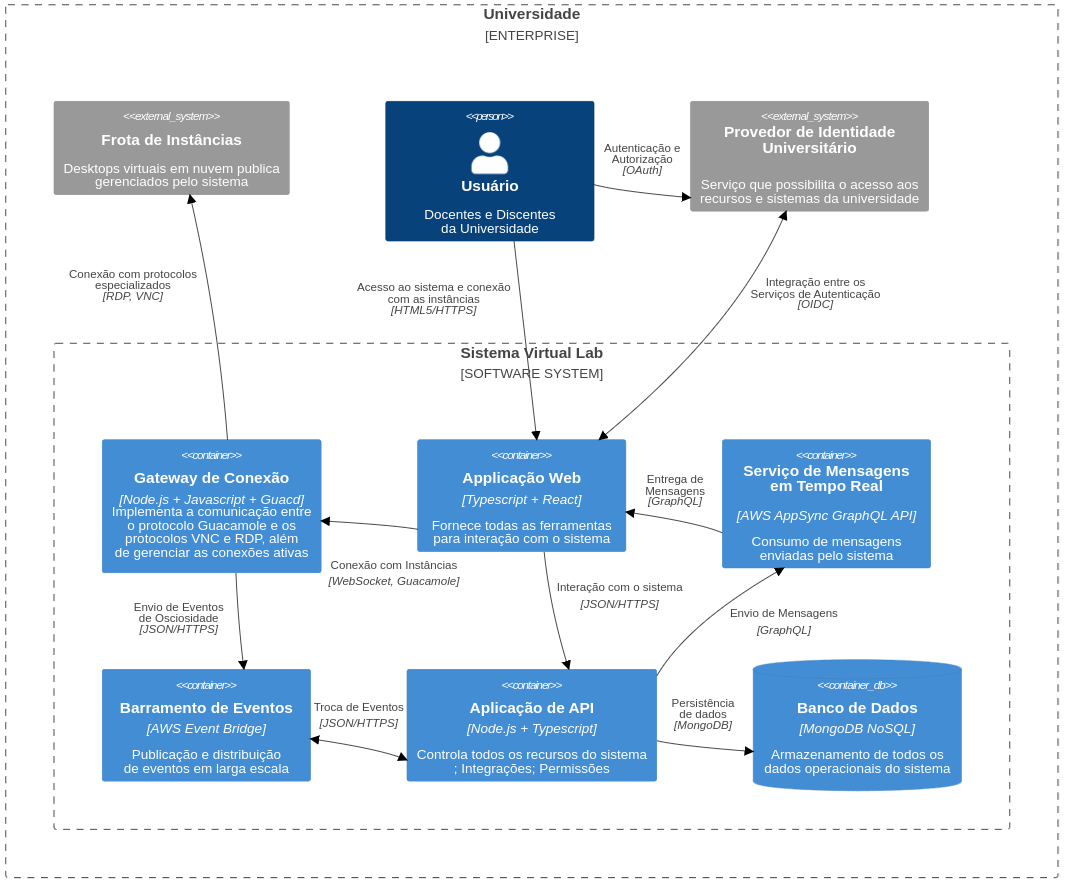
\includegraphics[width=\textwidth]{capitulos/2-metodologia/files/c4-container.png}
\fonte{Autoria Própria (2024)}
\end{figure}

A partir do diagrama de \textit{containers} do sistema, foi possível a estruturação interna de cada \textit{container} em componentes, que são as partes fundamentais para a implementação do sistema.
Nessa etapa, foram criados dois diagramas de componentes, um para a aplicação de API e outro para o gateway de conexão, que são as partes modeladas e implementadas por completo, enquanto os demais possuem apenas a definição de alto nível.

A \autoref{fig:diagramaC4ComponentesDaAPI} apresenta o diagrama de componentes da aplicação de API, que é responsável por orquestrar todas as operações do sistema que estão dispostas em quatro módulos de funcionalidades:

\begin{itemize}
    \item \textbf{Usuário}: Módulo responsável por gerenciar as informações e permisões dos usuários do sistema.

    \item \textbf{Instância}: Módulo responsável por gerenciar as instâncias do sistema e as operações que podem ser realizadas sobre elas.

    \item \textbf{Template de Instância}: Módulo responsável por gerenciar os templates de instância disponíveis no sistema e as operações que podem ser realizadas sobre eles.

    \item \textbf{Diversos}: Módulo responsável por gerenciar os recursos do sistema que servem de apoio para a aplicação \textit{web}, como a listagem de recursos recomendados utilizados na criação de templates de instância.

\end{itemize}

Nesse diagrama, a relação entre os módulos e os \glspl{port}, que são as interfaces da camada de aplicação, é explicitada. Porém, a explicação detalhada das comunicação não está presente pois cada módulo é composto por diversos casos de uso que são tratados de forma independente. Portanto, uma seta originada em um módulo e direcionada a um \gls{port} significa que pelo menos um caso de uso do módulo necessita de um \gls{adapter} que implementa a interface do \gls{port} para ser executado. 

A discussão sobre \glspl{port} e \glspl{adapter} é mais aprofundada na \autoref{sec:implementacao},
onde os padrões de arquitetura de código utilizados são apresentados.

\begin{figure}[H]
%\captionsetup{width=0.55\textwidth}%% Largura da legenda
\caption{Diagrama C4: Componentes da Aplicação de API}
\label{fig:diagramaC4ComponentesDaAPI}
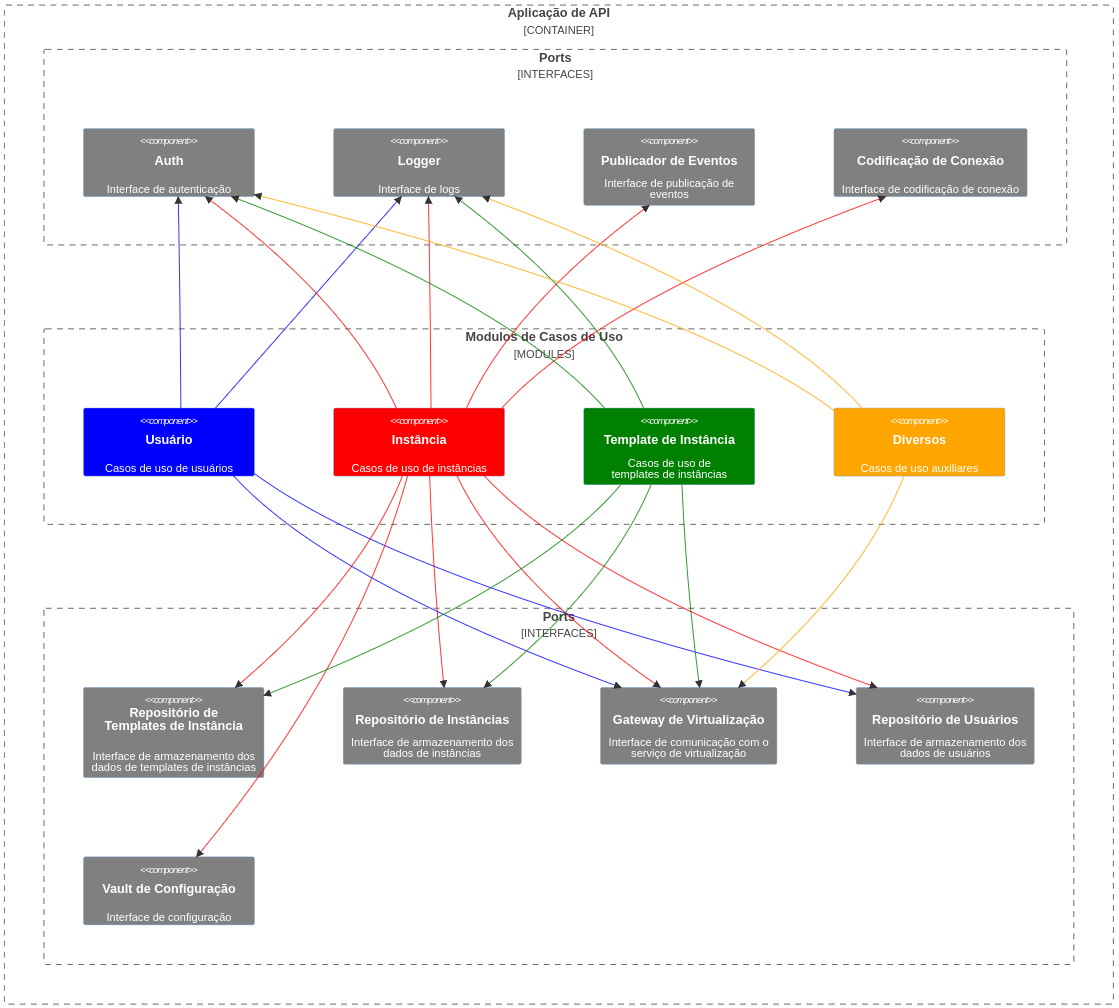
\includegraphics[width=\textwidth]{capitulos/2-metodologia/files/c4-component-api.png}
\fonte{Autoria Própria (2024)}
\end{figure}

O gateway de conexão é o componente responsável por intermediar a conexão entre o cliente web e as instâncias de máquinas virtuais. O diagrama de componentes do gateway de conexão é apresentado na \autoref{fig:diagramaC4ComponentesDoGateway}.

No gateway de conexão, além do gerenciamento das conexões com as instâncias de máquinas virtuais, o processo de identificação de conexões ativas e ociosas é realizado. Isso é de suma importância para o fluxo do sistema, já que seria difícil identificar a osciosidade através de alertas sensíveis às métricas de consumo dos recursos das instâncias.

Esse elo do sistema foi projetado para ser escalável horizontalmente, isto é, caso a demanda de conexões aumente, é possível adicionar mais instâncias do gateway de conexão para atender a demanda, sem a necessidade de alterar a arquitetura do sistema. Esse processo de escalabilidade é transparente para o usuário e também não afeta a disponibilidade do sistema.

Essa decisão foi tomada como uma medida de aprimoramento das perspectivas utilizadas no trabalho de \citet{edufirestick}, que é discutido na \autoref{sec:trabalhosRelacionados}. A escalabilidade horizontal é uma característica importante para sistemas que possuem uma demanda variável, como é o caso de sistemas de ensino e pesquisa, que podem ter picos de uso em determinados períodos do ano. Dessa forma o sistema pode "crescer" para atender a demanda e "encolher" quando a demanda diminuir para economizar custos.

\begin{figure}[H]
%\captionsetup{width=0.55\textwidth}%% Largura da legenda
\caption{Diagrama C4: Componentes do Gateway de Conexão}
\label{fig:diagramaC4ComponentesDoGateway}
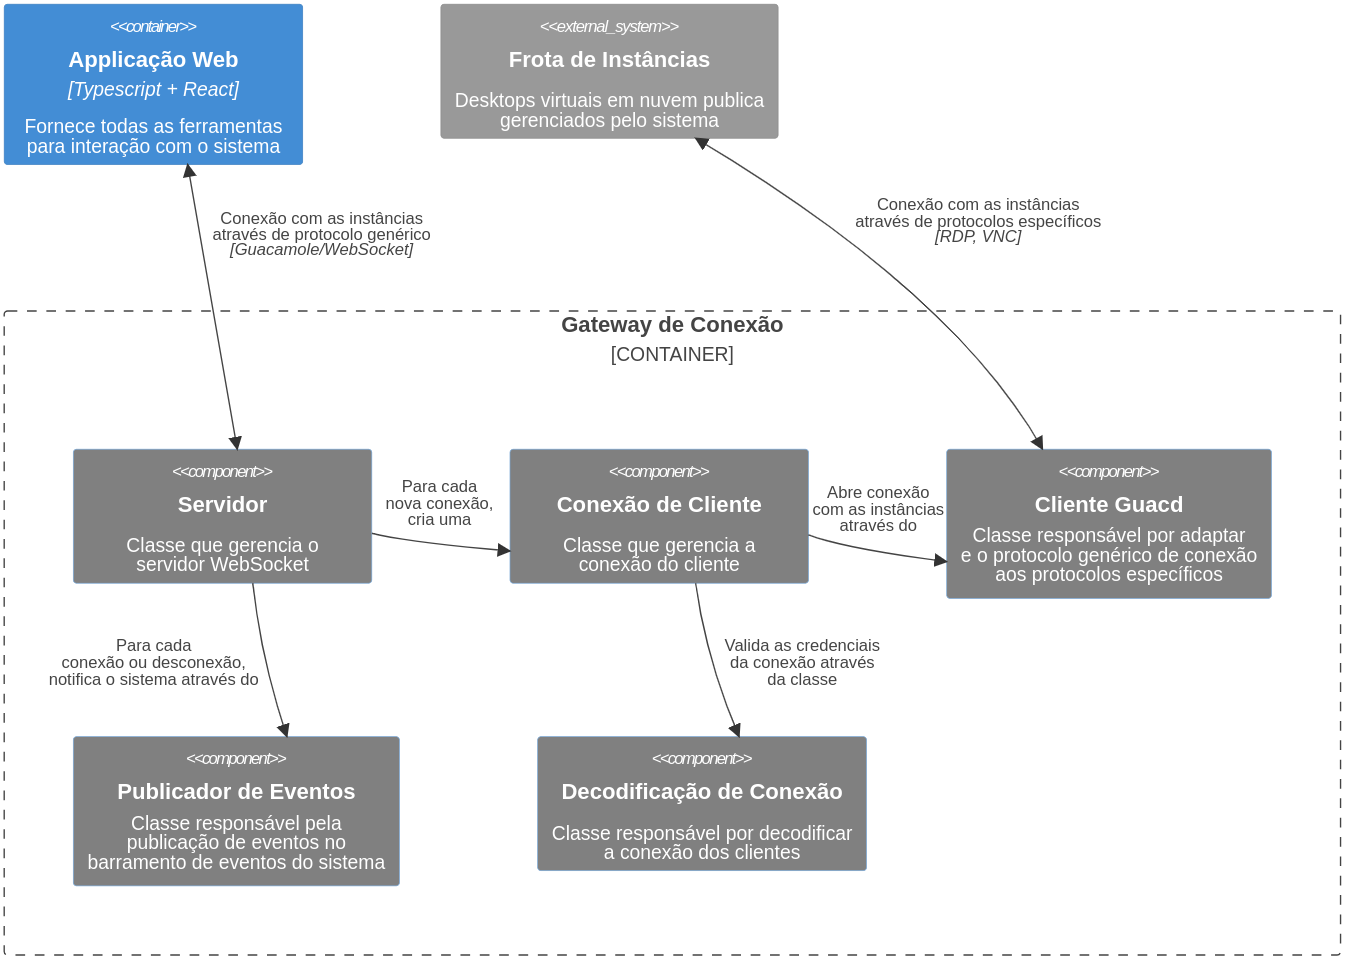
\includegraphics[width=\textwidth]{capitulos/2-metodologia/files/c4-component-connection-gateway.png}
\fonte{Autoria Própria (2024)}
\end{figure}

\section{Ferramentas e Tecnologias}
\label{sec:ferramentasETecnologias}

A \autoref{tab:ferramentasETecnologiasUtilizadas} apresenta uma lista de ferramentas, tecnologias e serviços utilizados na implementação do sistema. As versões utilizadas estão escritas de acordo com o padrão de versionamento semântico. \citep{semverdocs}

% Make de last column to be as wide as possible wrapping the text
\begin{longtable}{p{0.25\linewidth} p{0.15\linewidth} p{0.525\linewidth}}%% Ambiente longtable
\caption{Ferramentas e tecnologias utilizadas\label{tab:ferramentasETecnologiasUtilizadas}} \\%% Legenda e rótulo
\toprule
\textbf{Nome} & \textbf{Versão} & \textbf{Descrição} \\
\midrule
\endfirsthead%% Encerra cabeçalho da primeira página
\caption[]{Ferramentas e tecnologias utilizadas} \\%% Legenda
\multicolumn{3}{r}{\textbf{(continuação)}} \\
\toprule
\textbf{Nome} & \textbf{Versão} & \textbf{Descrição} \\
% \midrule
\endhead%% Encerra cabeçalho das demais páginas
% \midrule
\multicolumn{3}{r}{\textbf{(continua)}} \\
\endfoot%% Encerra rodapé das demais páginas
% \bottomrule
\\[-0.5\linha]
\caption*{\nomefonte: Autoria própria (2024)} \\
\endlastfoot%% Encerra rodapé da última página
Node.js \citep{nodejsdocs} & \textsuperscript{$\wedge$}18.19.0 & Ambiente de execução de javascript utilizado em todos os serviços de backend \\

\hline

ECMAScript \citep{ecmascriptdocs} & ES2020 & Especificação formal da linguagem javascript a qual o código escrito é compatível \\

\hline

Typescript \citep{typescriptdocs} & {$\leq$}5.4.0 & Extensão do Javascript que adiciona suporte para tipagem, utilizada na implementação de todos os serviços de backend e do cliente web do sistema \\

\hline

NPM \citep{npmdocs} & 10.2.3 & Gerenciador de dependências do Node.js \\

\hline

Shell Script \citep{shellscriptdocs} & \gls{n/a} & Linguagem de scripts utilizada para implementar a configuração automatizada das instâncias baseadas em LINUX \\

\hline

Windows PowerShell Script \citep{windowspowershelldocs} & 5 & Linguagem de scripts utilizada para implementar a configuração automatizada das instâncias baseadas em WINDOWS \\

\hline

Apache Velocity Template Language \citep{apachevelocitydocs} & 2.3 & Engine de templates utilizada para definir as permissões de conexão dos usuários ao serviços de notificações do servidor ao cliente \\

\hline

Markdown \citep{markdowndocs} & \gls{n/a} & Linguagem de marcação de texto utilizada na documentação do sistema \\

\hline

OpenAPI \citep{openapidocs} & 3.0.0 & Especificação para documentação de API. \\

\hline

Zod \citep{zoddocs} & \textsuperscript{$\wedge$}3.23.8 & Biblioteca utilizada para validar o conteúdo das requisições dos serviços \\

\hline

Prettier \citep{prettierdocs} & \textsuperscript{$\wedge$}3.3.1 & Utilitário utilizado para garantir a estilização do código. \\

\hline

Jest \citep{jestdocs} & \textsuperscript{$\wedge$}29.7.0 & Framework de teste para javascript \\

\hline

Eslint \citep{eslintdocs} & \textsuperscript{$\wedge$}8.56.0 & Utilitário de análise estática de código. \\

\hline

AWS CDK \citep{awscdkdocs} & 2.142.1 & Framework utilizado para definição dos componentes de infraestrutura como código \\

\hline

SST \citep{sstdocs} & 2.43.0 & Framework para construção de aplicações full-stack na AWS utilizando infraestrutura como código \\

\hline

Docusaurus \citep{docusaurusdocs} & \textsuperscript{$\wedge$}3.4.0 & Gerador de documentação em formato de site estático. \\

\hline

React \citep{reactdocs} & \textsuperscript{$\wedge$}18.0.0 & Biblioteca utilizada no desenvolvimento do cliente web do sistema \\

\hline

Stoplight Elements \citep{stoplightdocs} & \textsuperscript{$\wedge$}8.3.1 & Biblioteca utilizada para renderização da documentação da API. \\

\hline

Docker \citep{dockerdocs} & 24.0.5 & Ferramenta utilizada para a criação do ambiente isolado do gateway de conexão \\

\hline

Chakra UI \citep{chakrauidocs} & \textsuperscript{$\wedge$}2.8.2 & Biblioteca de componentes de interface utilizada no cliente web. \\

\hline

Apache Guacamole \citep{apacheguacamoledocs} & 1.5.3 & Utilizado para intermediar a conexão entre o cliente web e gateway de conexão. \\

\hline

Vite \citep{vitedocs} & \textsuperscript{$\wedge$}5.0.12 & Ferramenta responsável por gerenciar a implementação e o empacotamento do cliente web \\

\hline

MongoDB Atlas \citep{mongodbatlasdocs} & sdk \textsuperscript{$\wedge$}6.0.3 & Serviço de banco de dados não relacional utilizado para armazenar todos os dados do sistema. \\

\hline

AWS Amplify \citep{awsamplifydocs} & sdk \textsuperscript{$\wedge$}6.0.16 & Biblioteca com integrações facilitadas, uitilizada no cliente web para autenticação e conexão com AWS AppSync \\

\hline

AWS Lambda PowerTools \citep{awslambdapowertools} & \textsuperscript{$\wedge$}2.1.1 & Biblioteca utilizada para integrar a geração de logs dos serviços com o AWS CloudWatch \\

\hline

AWS AppSync \citep{awsappsync} & sdk \textsuperscript{$\wedge$}3.592.0 & Serviço utilizado para a comunicação em tempo real entre os serviçoes de backend e o cliente web \\

\hline

AWS Systems Manager \citep{awssystemsmanagerdocs} & sdk \textsuperscript{$\wedge$}3.592.0 & Serviço utilizado para armazenar as configurações do sistema. \\

\hline

AWS Event Bridge \citep{awseventbridgedocs} & sdk \textsuperscript{$\wedge$}3.592.0 & Serviço de gerenciamento de eventos utilizado como barramento de comunicação entre os serviços de backend. Oferece também a funcionalidade de agendamento de eventos, utilizado no sistema de desligamento automático de instâncias osciosas. \\

\hline

AWS CloudFormation \citep{awscloudformationdocs} & sdk \textsuperscript{$\wedge$}3.592.0 & Serviço utilizado para armazenar a definição dos componentes de infraestrutura como código \\

\hline

AWS Cognito \citep{awscognito} & sdk \textsuperscript{$\wedge$}3.592.0 & Serviço de gerenciamento de usuários e credenciais. Ele foi utilizado para gerenciar dados sensíveis, mantendo somente dados operacionais na integração com o banco de dados. \\

\hline

AWS Service Catalog \citep{awsservicecatalogdocs} & sdk \textsuperscript{$\wedge$}3.592.0 & Serviço de gerenciamento de modelos de IaC utilizado para o controle do ciclo de vida da instância e seus recursos dependentes \\

\hline

AWS CloudWatch \citep{awscloudwatchdocs} & sdk \textsuperscript{$\wedge$}3.592.0 & Serviço de monitoramento utilizado para agregar os logs dos sistemas. \\

\hline

AWS Lambda \citep{awslambdadocs} & sdk \textsuperscript{$\wedge$}3.592.0 & Serviço de computação serverless utilizado para executar o serviço de API e tratamento de eventos do sistema \\

\hline

AWS Api Gateway \citep{awsapigatewaydocs} & sdk \textsuperscript{$\wedge$}3.592.0 & Serviço gerenciado para criação de APIs serverless. \\

\hline

AWS Identity and Access Management \citep{awsiamdocs} & sdk \textsuperscript{$\wedge$}3.592.0 & Serivço utilizado para delimitação de todas as permissões atreladas aos componentes de infraestrutura do sistema \\

\hline

AWS S3 \citep{awss3docs} & sdk \textsuperscript{$\wedge$}3.592.0 & Serviço de armazenamento de objetos utilizado para servir o cliente web e armazenar todos os arquivos imutaveis do sistema \\

\hline

AWS CloudFront \citep{awscloudfrontdocs} & sdk \textsuperscript{$\wedge$}3.592.0 & Serviço de distribuição de conteúdo utilizado como camada distribuída de cache para os serviços \\

\hline

AWS Certificate Manager \citep{awscertificatemanagerdocs} & sdk \textsuperscript{$\wedge$}3.592.0 & Serviços utilizado para o gerenciamento dos certificados de domínio atrelados ao cliente web e à documentação \\

\hline

AWS Elastic Load Balancing \citep{awselasticloadbalancing} & sdk \textsuperscript{$\wedge$}3.592.0 & Balanceador de carga gerenciado utilizado para gerenciar as conexões entre o cliente web e o cluster de containers rodando o Gateway de conexão. \\

\hline

AWS Elastic Container Service \citep{awsecsdocs} & sdk \textsuperscript{$\wedge$}3.592.0 & Serviço utilizado para a implantação do gateway de conexão, no formato de cluster de containeres com escalabilidade previsível \\

\hline

AWS Elastic Container Registry \citep{awsecrdocs} & sdk \textsuperscript{$\wedge$}3.592.0 & Serviço utilizado para armazenar as imagens de container do gateway de conexão \\

\hline

AWS Simple Notification Service \citep{awssnsdocs} & sdk \textsuperscript{$\wedge$}3.592.0 & Serviço de publisher Subscriber utilizado para a transacionar as mensagens emitidas na criação de instâncias \\

\hline

AWS EC2 \citep{awsec2docs} & sdk \textsuperscript{$\wedge$}3.592.0 & Serviço central utilizado para gerenciar as instâncias, regras de conexão e as imagens de sistema operacional \\

\hline

\end{longtable}

O ecossistema de tecnologias utilizado foi escolhido a partir de alguns critérios, como a familiaridade com o ambiente de desenvolvimento, a facilidade de integração entre as ferramentas e a disponibilidade de documentação e comunidade de suporte.

Visto que a \gls{utfpr} já possui integração com a \gls{aws}, a escolha da provedor de nuvem pública foi trivial, já que a infraestrutura de serviços da \gls{aws} é também utilizada em projetos a nível empresarial e acadêmico a nível global, oferecendo um portfólio extenso de serviços que atendem as necessidades do sistema.

O SST foi escolhido como um facilitador tanto para o fluxo de desenvolvimento local quanto para a definição de todos os componentes de arquiteura como código. A ferramenta disponibiliza componentes de alto nível que já implementam as melhores práticas de segurança e controle de custos. Além disso, o SST estabelece uma conexão entre os serviços da \gls{aws}, como as funções Lambda, e o código escrito localmente, fazendo com que seja possível testar e depurar o código no seu ambiente próprio de implantação.

O \gls{guacamole} foi escolhido como intermediador da conexão entre o cliente web e as instâncias de máquinas virtuais, porque trata-se de uma ferramenta de código aberto bem estabelecida que fornece os componentes necessários para a conexão remota a partir de um navegador de internet. Além disso, ele é compatível com os protocolos de conexão remota utilizados no trabalho. No contexto do desenvolvimento do sistema, o \gls{guacamole} foi utilizado de forma customizada. Apenas \textit{daemon} que implementa a conexão remota, o componente web que renderiza a interface de conexão e o protocolo de comunicação em si foram utilizados.

Essa customização foi necessária para que o sistema pudesse controlar todos os aspectos de interface e conexão, caso contrário, seria necessário utilizar a aplicação web já existente do \gls{guacamole}. Se esse fosse o caso, a customização do sistema dependeria de um conjunto de regras de negócio implementadas diretamente no \gls{guacamole}, o que dificultaria a manutenção e a evolução do sistema.

\section{Modelo de Dados}
\label{sec:modeloDeDados}

Aqui foi realizado o projeto do modelo de dados do sistema, que é a representação das entidades e relacionamentos centrais do sistema. O modelo de dados foi construído a partir dos requisitos funcionais do sistema, casos de uso e desdobramentos da arquitetura do sistema, de forma a garantir que todas as informações necessárias para o funcionamento do sistema estejam presentes. 

No contexto de sistemas de software altamente dependentes da infraestrutura de nuvem, o modelo de dados precisa levar em consideração as características de funcionamento e dados disponibilizados pelos serviços de nuvem, como a \gls{aws}. Esse é o motivo pelo qual essa seção é apresentada após a discussão sobre a arquitetura do sistema e decisão das tecnologias utilizadas.

O modelo de dados foi elaborado a partir da especificação das entidades funcionais do sistema. A \autoref{fig:diagramaDeClasses} apresenta o diagrama de classes, onde cada classe é uma entidade funcional do sistema, exceto pelas interfaces representadas que apenas indicam modelos de dados mais complexos.

\begin{figure}[H]
    %\captionsetup{width=0.55\textwidth}%% Largura da legenda
\caption{Diagrama de Classes do Sistema}
\label{fig:diagramaDeClasses}
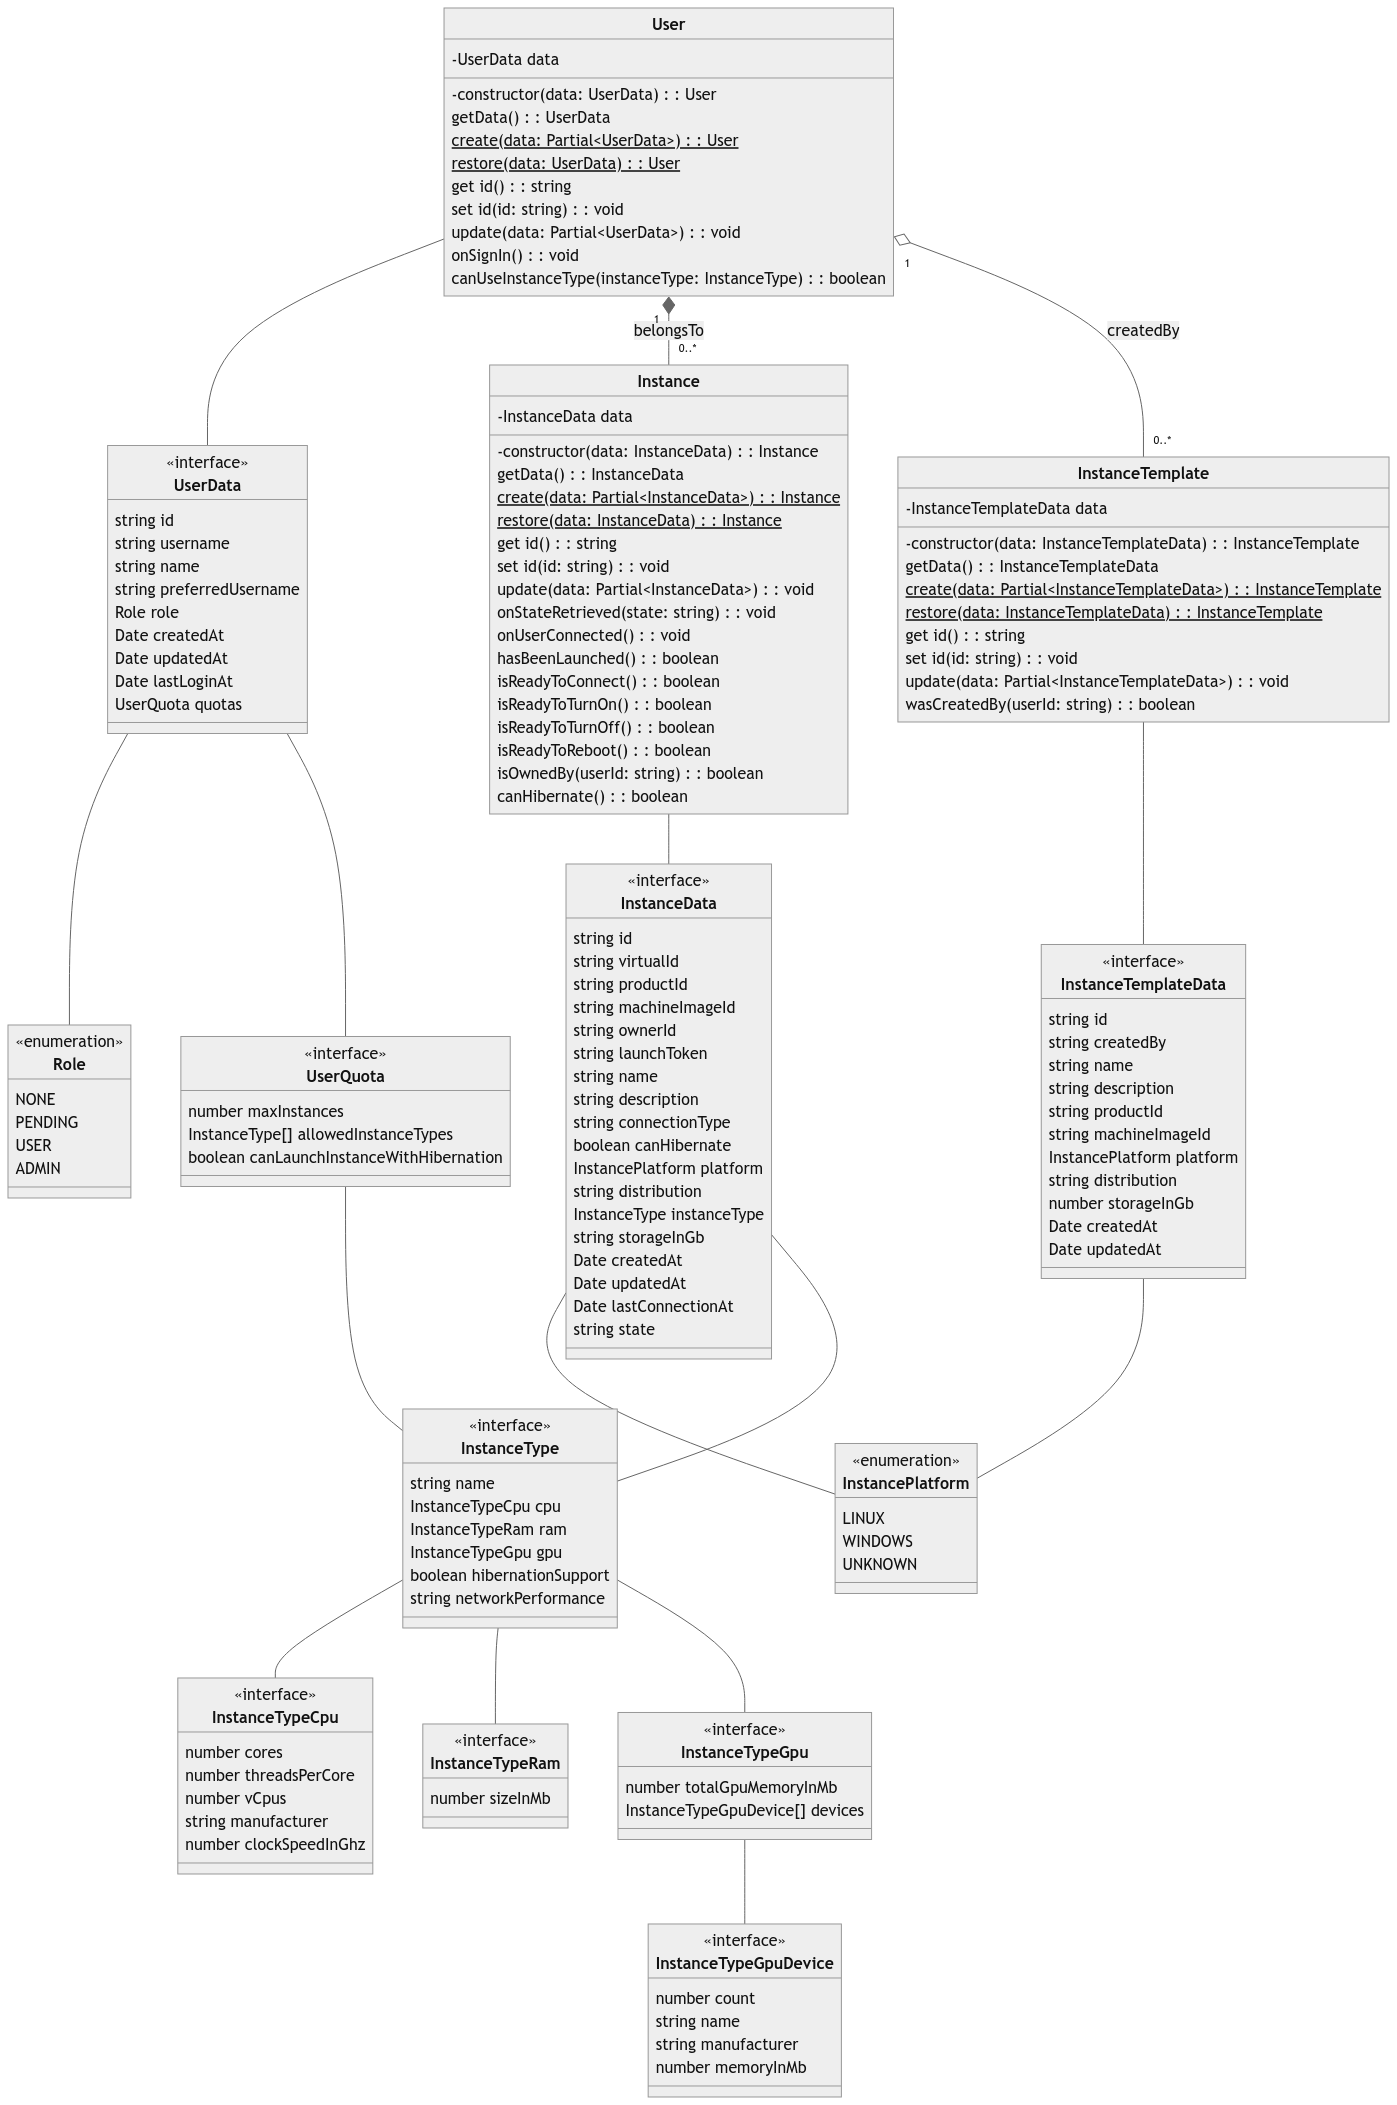
\includegraphics[width=\textwidth]{capitulos/2-metodologia/files/class-diagram.png}
\fonte{Autoria Própria (2024)}
\end{figure}

\section{Implementa\c{c}\~ao}
\label{sec:implementacao}

Essa seção apresenta os aspectos pertinentes ao processo de desenvolvimento do sistema, passando pela organização do repositório de código, dos serviços e componentes, dos componentes de infraestrutura e dos testes automatizados. É importante ressaltar que as implementações seguem as ferramentas e tecnologias apresentadas na \autoref{sec:ferramentasETecnologias}.

\subsection{Repositório de código}
\label{subsec:repositorioDeCodigo}

O repositório de código foi organizado através de uma estrutura de \textit{monorepo}, onde o código fonte de todos os serviços e componentes de infraestrutura como código são versionados dentro de um único repositório de código fonte. 

A utilização dessa abordagem com o uso do framework SST facilitou o desenvolvimento integrado de todas as pertes do sistema desde o início, diminuindo as chances de problema no processo de integração entre partes separadas. Além disso, foi possível desenvolver conjuntos bem definidos de funcionalidades em pacotes envolvendo interfaces de usuário, regras de negócio e componentes de infraestrutura.

A estrutura de alto nível do repositório de código foi organizada da seguinte forma:

\dirtree{%
.1 /.
.2 \textbf{\_\_tests\_\_} \ldots{} \begin{minipage}[t]{\textwidth}
Configurações do ciclo de vida dos testes
\end{minipage}.
.2 \textbf{.github}.
.3 \textbf{workflows}.
.4 \textbf{ci.yml} \ldots{} \begin{minipage}[t]{0.7\textwidth}
Implementação do fluxo de integração contínua
\end{minipage}.
.2 \textbf{packages} \ldots{} \begin{minipage}[t]{\textwidth}
Implementação dos serviços do sistema
\end{minipage}.
.3 \textbf{api} \ldots{} \begin{minipage}[t]{\textwidth}
Aplicação de API
\end{minipage}.
.3 \textbf{app-sync-api} \ldots{} \begin{minipage}[t]{\textwidth}
Serviço de Mensagens em Tempo Real
\end{minipage}.
.3 \textbf{client} \ldots{} \begin{minipage}[t]{\textwidth}
Cliente Web 
\end{minipage}.
.3 \textbf{connection-gateway} \ldots{} \begin{minipage}[t]{\textwidth}
Gateway de Conexão
\end{minipage}.
.3 \textbf{docs} \ldots{} \begin{minipage}[t]{\textwidth}
Documentação
\end{minipage}.
.2 \textbf{stacks} \ldots{} \begin{minipage}[t]{\textwidth}
Definição de infraestrutura como código
\end{minipage}.
.3 \textbf{config} \ldots{} \begin{minipage}[t]{\textwidth}
Configurações de implantação
\end{minipage}.
.3 \textbf{products} \ldots{} \begin{minipage}[t]{0.65\textwidth}
Base de stacks para cada sistema operacional
\end{minipage}.
.3 \textbf{scripts} \ldots{} \begin{minipage}[t]{0.7\textwidth}
Scripts de preparação para cada sistema operacional
\end{minipage}.
.2 \textbf{.env.example} \ldots{} \begin{minipage}[t]{\textwidth}
Exemplo das variáveis de ambiente
\end{minipage}.
.2 \textbf{package.json} \ldots{} \begin{minipage}[t]{0.7\textwidth}
Gerenciamento das dependências compartilhadas e de infraestrutura
\end{minipage}.
.2 \textbf{sst.config.ts} \ldots{} \begin{minipage}[t]{0.6\textwidth}
Configuração do framework SST e injeção das stacks de infraestrutura
\end{minipage}.
}

\hfill\break

A cada \textit{commit} no repositório, um fluxo de integração contínua foi acionado executando uma sequência de operações que auxiliaram na validação do código entregue. O fluxo de integração contínua foi implementado utilizando o \textit{GitHub Actions}, que é uma ferramenta de automação de \textit{workflows} disponibilizada pelo GitHub. O \autoref{cap:apendiceb} apresenta o código do fluxo de integração contínua.


\subsection{Banco de Dados}
\label{subsec:bancoDeDados}

O banco de dados utilizado no sistema foi o \textit{MongoDB Atlas}, que é um serviço de banco de dados não relacional orientado a documentos, especificado também na \autoref{tab:ferramentasETecnologiasUtilizadas}.

O modelo dos dados foi implementado utilizando a biblioteca \textit{mongodb}, que é um \textit{Object Data Modeling} (ODM) para o MongoDB e Node.js. A biblioteca \textit{mongodb} fornece uma interface de alto nível para a interação com o banco de dados, permitindo realizar operações tipadas.

Esse tipo de banco de dados não necessita de um configuração prévia do esquema dos dados, e por isso não foi necessário a implementação de migrações de banco de dados. Por outro lado a consistência dos dados deve ser garantida através de boas práticas de programação e validações, bem como mencionado nos princípios de modelagem no início da \autoref{sec:modelagemDoSistema}.

Não foram adicionados índices adicionais ao banco de dados. O índice padrão do \textit{mongodb}, que faz do campo \textit{id} um valor único e incremental, foi suficiente para garantir a performance das operações de leitura e escrita.

\subsection{Serviço de Mensagens em Tempo Real}
\label{subsec:servicoDeMensagensEmTempoReal}

Este serviço foi implementado utilizando o \textit{AWS AppSync}, que é um serviço de comunicação em tempo real da \gls{aws} que permite a criação de APIs GraphQL com suporte para padrões de comunicação em tempo real executando sobre o protocolo \textit{WebSocket}.

A implementação do serviço foi realizada em três frentes. A primeira foi a definição do esquema \textit{GraphQL} com as operação de \textit{Subscription} que são utilizadas pelos clientes para se inscreverem em canais de comunicação específicos, além dos \textit{resolvers} que são funções escritas na linguagem \textit{VTL} e que foram utilizadas para o processo de autorização das requisições. A segunda etapa foi a implementação das interfaces utilizada pelo servidor para enviar as mensagens para os clientes e pelos clientes para se inscreverem nos canais de comunicação. A terceira e última etapa consistiu na implementação dos recursos de infraestrutura necessários para o funcionamento do serviço, como a definição de permissões, conexão do esquema e dos \textit{resolvers}.

Para garantir o isolamento dos canais de comunicação e evitar que usuários mal intencionados possam acessar informações de outros usuários, os usuários foram habilitados de realizar a inscrição apenas no canal com o seu próprio identificador. Esse identificador é gerado no momento da criação da conta do usuário e é utilizado para garantir a unicidade do canal de comunicação.

A implementação da interface feita no cliente web foi intermediada pela da biblioteca \textit{AWS Amplify}, que é uma biblioteca de integração com os serviços da \gls{aws} para aplicações web e móveis.

\subsection{Barramento de Eventos}
\label{subsec:barramentoDeEventos}

O barramento de eventos foi implementado utilizando o \textit{AWS Event Bridge}, que é um serviço de gerenciamento de eventos da \gls{aws} que permite a comunicação entre os serviços de forma assíncrona e escalável. A implementação é baseada na criação de regras de eventos que são acionadas quando um evento específico é publicado no barramento. Ele foi escolhido para ser o principal meio de comunicação entre os serviços de backend, já que ele oferece integração com diversos serviços da \gls{aws} e também funcionalidade de agendamento de eventos, que foi utilizada no sistema de desligamento automático de instâncias ociosas.

A implementação do barramento de eventos foi realizada em duas frentes. A primeira foi a definição das regras de eventos que são acionadas quando um evento específico é publicado no barramento. A segunda etapa foi a implementação dos recursos de infraestrutura necessários para o funcionamento do serviço, juntamente com a conexão entre os serviços de backend e o barramento de eventos.

Para publicar eventos no barramento, os serviços de \textit{backend} utilizaram o prório \textit{SDK} da \gls{aws}.

\subsection{Gateway de Conexão}
\label{subsec:gatewayDeConexao}

Esse serviço foi modelado para intermediar a conexão entre o cliente web e as instâncias de máquinas virtuais, e sua implementação foi baseada na estrutura de um servidor \textit{websocket}, onde as conexão são persistidas e mantidas abertas para permitir a comunicação.

A implementação do código foi baseada no diagrama da \autoref{fig:diagramaC4ComponentesDoGateway}, onde o serviço foi dividido em cinco classes de responsabilidades específicas.

A primeira classe, \textit{Server} ficou responsável por gerenciar o ciclo de vida do servidor \textit{websocket}, aceitando novas conexões e mantendo as conexões ativas. A segunda classe, \textit{ClientConnection} ficou responsável por implementar as operações pertinentes a troca de dados entre o cliente que iniciou a conexão e a classe \textit{guacdClient} que é a terceira classe, responsável especificamente por interagir com o binário \textit{guacd} do \gls{guacamole}, que é nativamente implementado na linguagem C. A quarta classe, \textit{Crypt} ficou responsável por implementar as operações de descriptografia do token de conexão, que é gerado pela aplicação de API e encaminhado através do cliente web. A quinta e última classe é o \textit{EventPublisher}, que é uilizado pela classe \textit{Server} para publicar eventos de conexão e desconexão no barramento de eventos. Eventos estes que são consumidos por funções \textit{Lambda} dentro do domínio da aplicação de API que agendam o desligamento automático de instâncias ociosas.

O algoritmo de criptografia utilizado tanto pela classe \textit{Crypt} para descriptografar o token de conexão, quanto pela aplicação de API para criptografar o token de conexão, foi o algoritmo de criptografia simétrica \textit{AES-256}. Esse algoritmo foi utilizado em \textit{Cipher Block Chaining (CBC)}, que é um modo de funcionamento que evita que padrões repetidos no texto claro sejam visíveis no texto cifrado.

Como o \textit{guacd}, binário do \gls{guacamole}, precisa ser executado no mesmo ambiente que as classes do serviços, foi necessário a criação de um ambiente completo para a execução do serviço, através de um \textit{container} \textit{Docker}. O conteiner utilizou a imagem oficial fornecida pelo \gls{guacamole} somente com o binário, como também a imagem oficial do \textit{Node.js} para a execução do código do serviço, dessa forma foi possível garantir que o serviço se comportaria da mesma maneira em qualquer ambiente. Quando o \textit{container} é iniciado, a ferramenta \textit{supervisord} gerencia a execução dos processos do \textit{guacd} e do serviço, permitindo o controle e monitoramento dos processos através de um único ponto de entrada.

\subsection{Aplicação de API}
\label{subsec:aplicacaoDeAPI}

Esse serviço é o ponto central de comunicação entre o cliente web e os demais serviços de backend. 
Ele foi implementado utilizando \textit{typescript} e \textit{Node.js} e padrões de arquitetura de código e de projeto para que fosse possível expandir o sistema de maneira incremental, sem que a complexidade do código aumentasse de forma descontrolada.

Para isso, o padrão de arquitetura de código \textit{Arquitetura Hexagonal}, conhecida também como \textit{Ports and Adapters}, foi utilizado. Esse padrão de arquitetura de código é baseado na separação das responsabilidades do código em camadas, onde a camada de aplicação é o núcleo do sistema e as camadas de infraestrutura e de interface são adaptadores que permitem a comunicação com o núcleo. Além disso, essa arquitetura permitiu que o conceito de inversão de dependência fosse aplicado, criando uma separação clara entre as regras de negócio e a implementação dos serviços.

A estrutura do serviço foi organizada da seguinte forma:

\dirtree{%
.1 /packages/api.
.2 application \ldots{} \begin{minipage}[t]{0.65\textwidth}
Camada que contém as regras de negócio do sistema, implementadas em classes de casos de uso
que orquestram as entidades do domínio do sistema e os \textit{ports} de comunicação
\end{minipage}.
.3 use-cases.
.4 instance.
.5 \_\_tests\_\_.
.5 launch-instance.ts.
.4 instance-template.
.4 misc.
.4 user.
.3 auth.ts \ldots{} \begin{minipage}[t]{0.7\textwidth}
Exemplo de \gls{adapter} de autenticação que define as operações de autenticação do sistema, sem implementar a lógica de autenticação
\end{minipage}.
.2 domain \ldots{} \begin{minipage}[t]{0.75\textwidth} % 0.75\textwidth
Camada de domínio da aplicação, que contém a implementação das classes modeladas e dos protocolos de dados utilizados em todas as outras camadas do sistema
\end{minipage}.
.3 dtos.
.3 entities.
.4 instance-template.ts.
.4 instance.ts.
.4 user.ts.
.2 infrastructure \ldots{} \begin{minipage}[t]{0.65\textwidth}
Camada de infraestrutura, que implementa as interfaces definidas na camada de aplicação de modo a realizar a comunicação com os serviços externos
\end{minipage}.
.3 auth.
.4 cognito-auth.ts \ldots{} \begin{minipage}[t]{0.5\textwidth}
Exemplo de implementação do \textit{port} de autenticação utilizando o serviço de autenticação da \gls{aws}
\end{minipage}.
.4 in-memory-auth.ts \ldots{} \begin{minipage}[t]{0.5\textwidth}
Exemplo de implementação do \textit{port} de autenticação utilizando lógica isolada em memória, com o objetivo de ser utilizado em testes unitários
\end{minipage}.
.2 interfaces \ldots{} \begin{minipage}[t]{0.7\textwidth}
Camada de interfaces, que utiliza todas as outras camadas para implementar os pontos de acesso do sistema
\end{minipage}.
.3 api \ldots{} \begin{minipage}[t]{0.8\textwidth}
Implementação de todos os endpoits da API, compatíveis para serem executados em funções \textit{Lambda}
\end{minipage}.
.3 events \ldots{} \begin{minipage}[t]{0.7\textwidth}
Implementação dos pontos de entrada que consomem os eventos do barramento de eventos
\end{minipage}.
.3 jobs \ldots{} \begin{minipage}[t]{0.8\textwidth}
Implementação de pontos de entrada que realizam operações assíncronas, como as rotinas de atualização de alguns recursos no momento de implantação do código
\end{minipage}.
}

\subsection{Cliente Web}
\label{subsec:clienteWeb}

O cliente web foi implementado utilizando \textit{typescript} e \textit{React} como a base tecnológica principal. Para a construção da interface a biblioteca de componentes \textit{Chakra UI} foi utilizada, pois ela oferece uma série de componentes customizáveis que implementam boas práticas de acessibilidade e permitem um controle sobre a apresentação dos componentes em diferentes formatos de tela.

As páginas e contexto do cliente web foram estruturados em componentes reutilizáveis, que são utilizados em diferentes partes do sistema. Bem como a camada que lida com a troca de dados com a aplicação de API, que foi implementada utilizando a biblioteca \textit{ReactQuery}, que é uma biblioteca de gerenciamento de estado que fornece uma abstração sobre a chamadas dos \textit{endpoints} da API, permitindo o cache local com tempo de expiração pré-definido e também o consumo dos recursos da API de forma equilibrada, evitando requisições redundantes ou excessivas.


\subsection{Documentação}
\label{subsec:documentacao}

A documentação foi desenvolvida utilizando o \textit{Docusaurus}, que é um gerador de documentação em formato de site estático. Com ele foi possível escrever a documentação em formato de \textit{Markdown} com suporte a componentes de \textit{React}, a mesma tecnologia utilizada no cliente web, para então gerar um site estático com a documentação do sistema.

Ao utilizar essa ferramenta, o processo de documentação ficou focado na produção dos conteúdos de ajuda ao usuário e também na documentação técnica do sistema, sem a preocupação da estrutura do sistema de documentação, já que é uma parte acoplada ao sistema que não precisa de novas funcionalidades, precisa apenas de complementos textuais.

Para que a documentação das rotas de api pudessem ser listadas de forma automática, foi utilizado o \textit{Stoplight Elements}, que é uma biblioteca que permite a renderização de documentação de API em formato de componente \textit{React} a partir de um arquivo de especificação \textit{OpenAPI} também gerado automaticamente dentro do processo de sintetização da stack da Aplicação de API, onde as rotas são definidas.

A \autoref{fig:docsintroduction} apresenta a página inicial da documentação do sistema e a \autoref{fig:docsapi} apresenta um exemplo de rota documentada.

\begin{figure}[H]
%\captionsetup{width=0.55\textwidth}%% Largura da legenda
\caption{Página inicial da documentação do sistema}
\label{fig:docsintroduction}
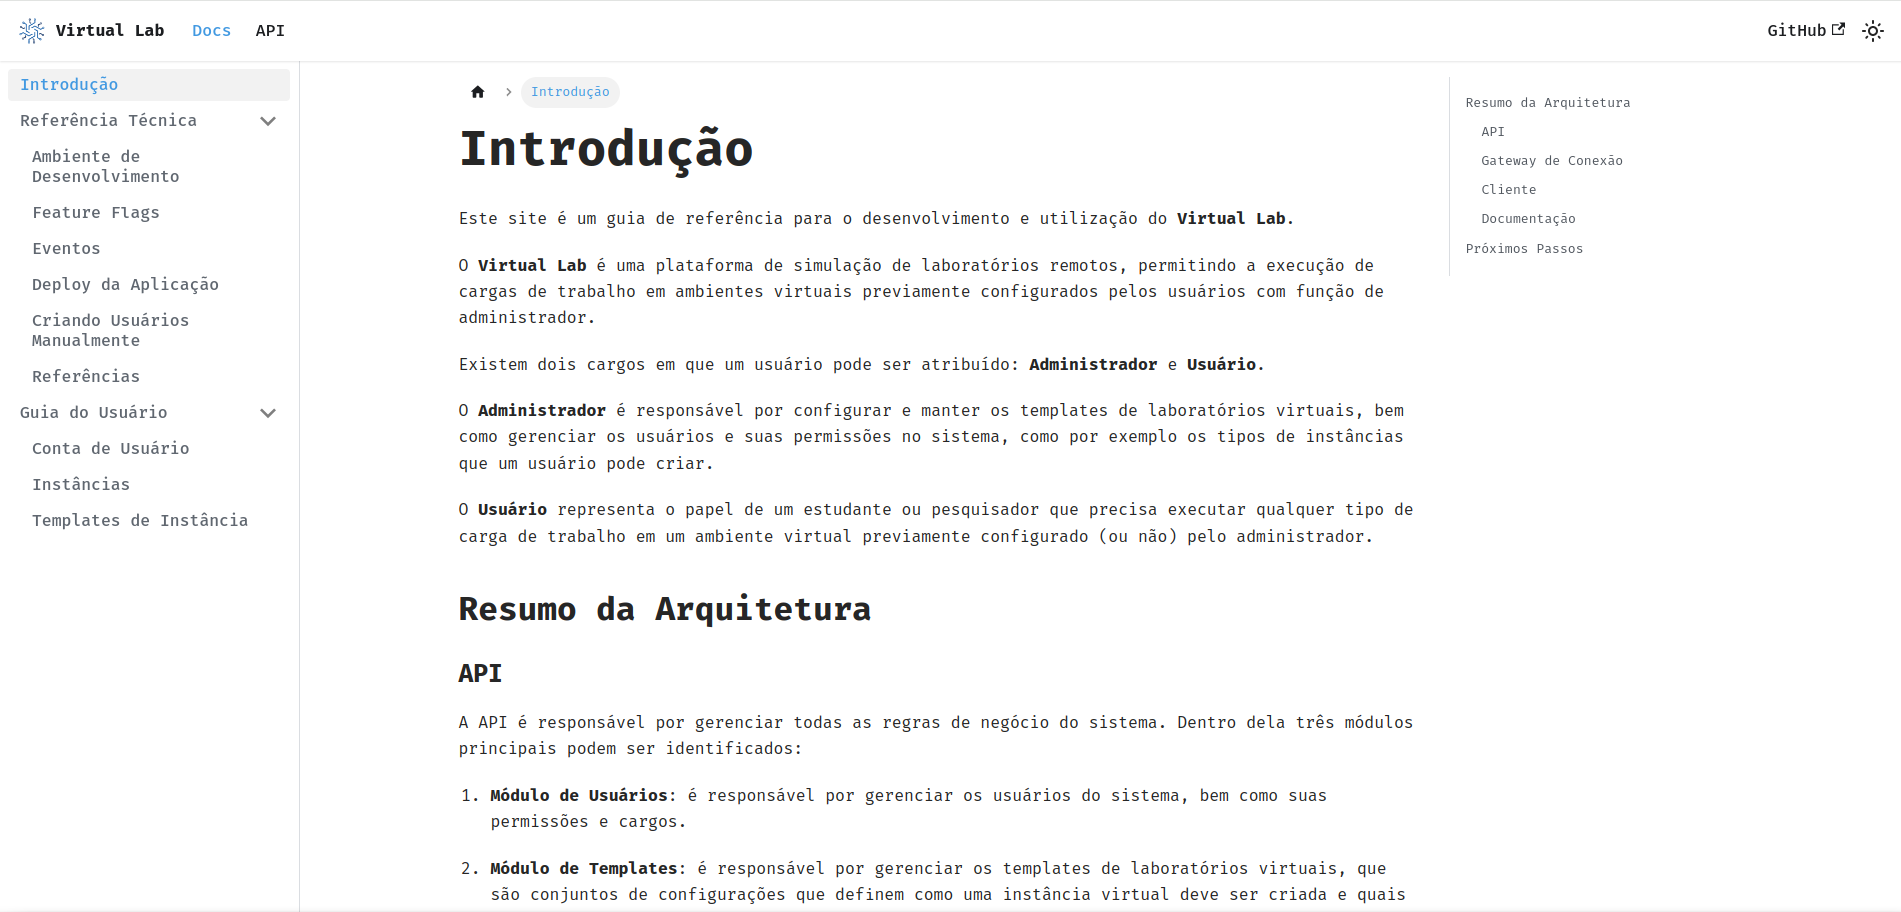
\includegraphics[width=\textwidth]{capitulos/2-metodologia/files/docs-introduction.png}
\fonte{Autoria Própria (2024)}
\end{figure}

\begin{figure}[H]
%\captionsetup{width=0.55\textwidth}%% Largura da legenda
\caption{Documentação da rota de API: Listar Instâncias}
\label{fig:docsapi}
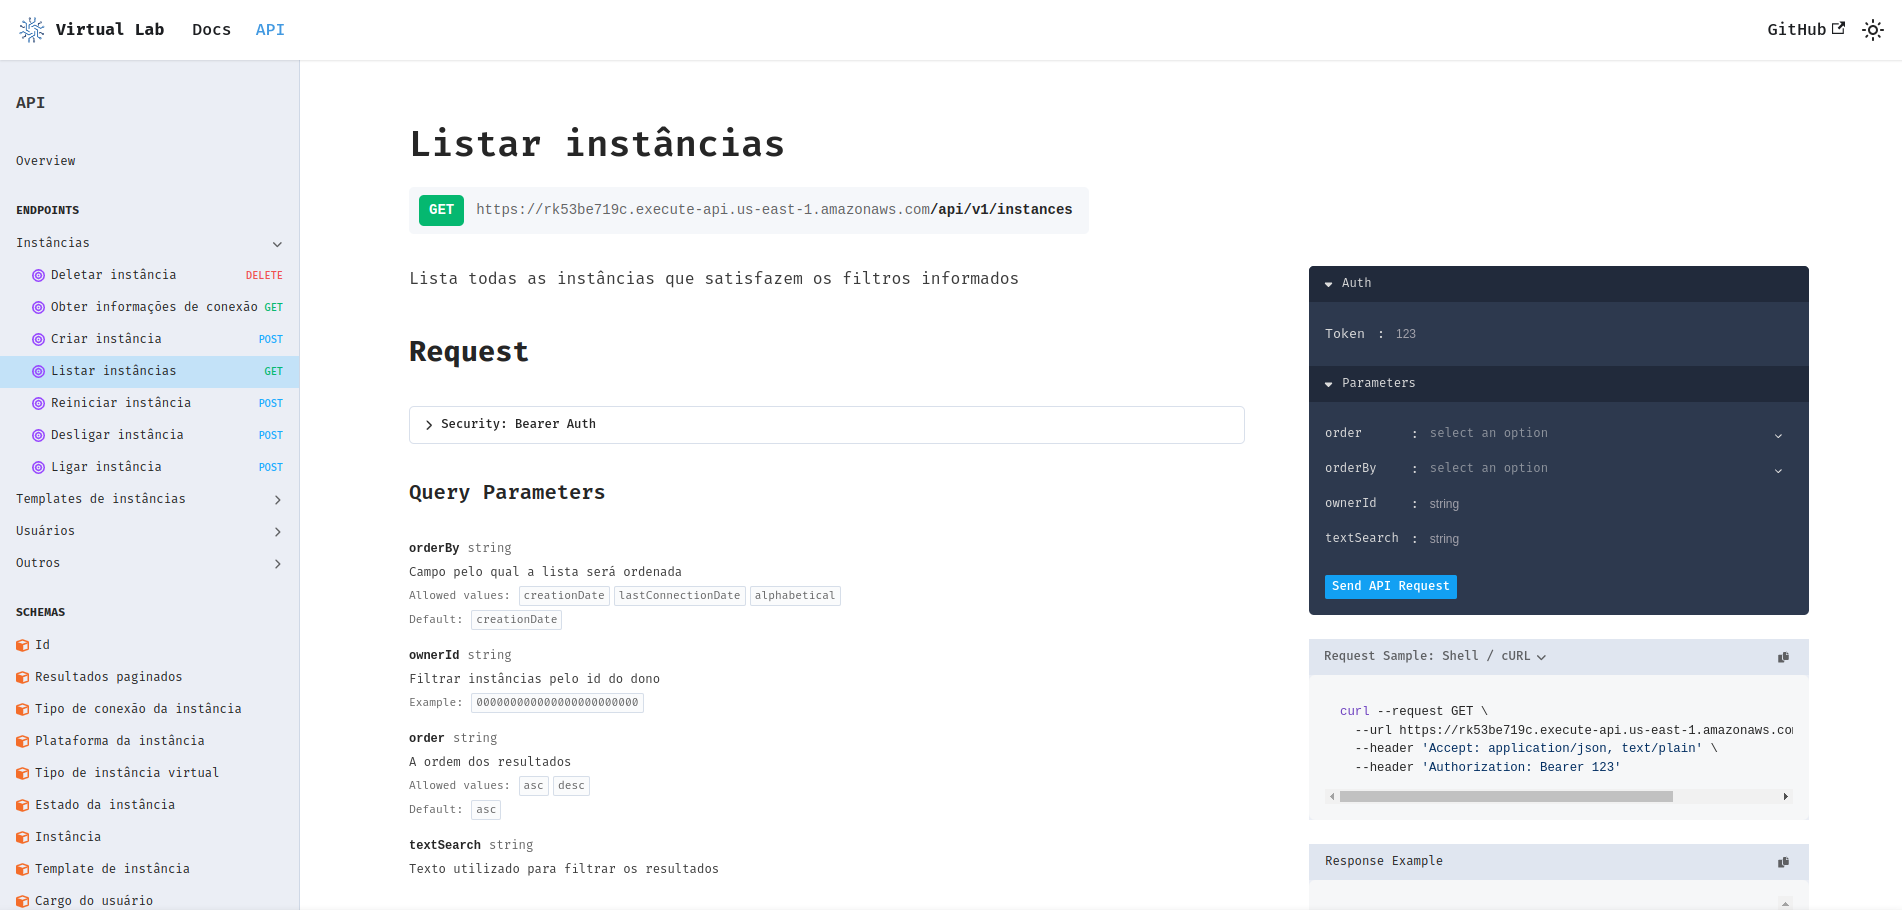
\includegraphics[width=\textwidth]{capitulos/2-metodologia/files/docs-api.png}
\fonte{Autoria Própria (2024)}
\end{figure}

\subsection{Testes Automatizados}
\label{subsec:testesAutomatizados}

Testes exaustivos não garantem a ausência de falhas, mas podem reduzir a probabilidade de falhas críticas. \citep{pressman2016}

Os testes do sistema foram realizados de duas formas, a primeira através de testes unitários automatizados e a segunda através da execução manual de um teste \textit{end-to-end} percorrendo os caminhos críticos da aplicação.

Os testes unitários foram implementados através do framework \textit{Jest} a fim validar de forma satisfatória todos os casos de uso dos serviços de backend. Como visto anteriormente, a estrutura do projeto já foi planejada para facilitar a escrita de testes utilizando \glspl{adapter} implementados especificamente para reproduzir o comportamento dos serviços reais da camada de infraestrutura.

A seguir os testes unitários dos casos de usos mais importantes implementados serão listados, com suas condições iniciais e resultados esperados. O \autoref{cap:apendicea} apresenta o relatório de cobertura dos testes por arquivo com os resultados obtidos.

\begin{table}[h]
\caption{Testes unitários do caso de uso: Desligar instância ociosa}
\label{tab:testeDesligarInstanciaOciosa}
\begin{tabularx}{\textwidth}{p{0.45\textwidth} p{0.5\textwidth}}
\toprule
\textbf{Condição inicial} & \textbf{Resultado esperado} \\ \midrule

Quando a entrada do caso de uso é inválida & Deve retornar um erro de validação \\ \hline

Quando a instância indicada não existe & Não deve realizar nenhuma ação \\ \hline

Quando a instância indicada existe e pertence a um usuário & Deve desligar a instância \\ 

\bottomrule
\end{tabularx}
\fonte{Autoria própria (2024)}%% Fonte
\end{table}

Os casos de teste da \autoref{tab:testeDesligarInstanciaOciosa} são importantes para garantir que quando o agendamento para desligamento é acionado, a instância de fato será desligada, evitando assim que recursos sejam desperdiçados e que o usuário consiga acessar a instância de outro local diferente do cliente web do sistema.


\begin{table}[h]
\caption{Testes unitários do caso de uso: Deletar instância}
\label{tab:testeDeletarInstancia}
\begin{tabularx}{\textwidth}{p{0.45\textwidth} p{0.5\textwidth}}
\toprule
\textbf{Condição inicial} & \textbf{Resultado esperado} \\ \midrule

Quando a entrada do caso de uso é inválida & Deve retornar um erro de validação \\ \hline

Quando o usuário não tem permissão para deletar a instância & Deve retornar um erro de permissão \\ \hline

Quando a instância indicada não existe & Não retornar um erro de instância não encontrada \\ \hline

Quando o cargo do usuário não é administrador e a instância pertence a outro usuário & Deve retornar um erro de permissão \\ \hline

Quando o usuário tem permissão para deletar a instância & Deve deletar a instância e todos os recursos associados \\

\bottomrule
\end{tabularx}
\fonte{Autoria própria (2024)}%% Fonte
\end{table}

Na \autoref{tab:testeDeletarInstancia} os testes também são importantes para o gerenciamento correto dos recursos da nuvem, já que é preciso deletar o registro do objeto no banco de dados e também todos os recursos que foram criados na nuvem, como a instância, o grupo de segurança, volumes de armazenamento, estes que se ficarem foram de uso, podem gerar custos desnecessários e difíceis de rastrear.


\begin{table}[h]
\caption{Testes unitários do caso de uso: Obter informações de conexão com instância} 
\label{tab:testeObterInformacoesDeConexaoComInstancia}
\begin{tabularx}{\textwidth}{p{0.45\textwidth} p{0.5\textwidth}}
\toprule
\textbf{Condição inicial} & \textbf{Resultado esperado} \\ \midrule

Quando a entrada do caso de uso é inválida & Deve retornar um erro de validação \\ \hline

Quando o usuário não está habilitado para acessar o sistema & Deve retornar um erro de permissão \\ \hline

Quando a instância indicada não existe & Deve retornar um erro de instância não encontrada \\ \hline

Quando o sistema não consegue obter a senha da instância & Deve retornar um erro interno \\ \hline

Quando o usuário não é o dono da instância e não é administrador & Deve retornar um erro de permissão \\ \hline

Quando o usuário tem acesso à instância e a mesma ainda não está pronta para conexão & Deve retornar um erro de violação do caso de uso \\ \hline

Quando o usuário tem acesso à instância e a mesma não está ligada & Deve retornar um erro de violação do caso de uso \\ \hline

Quando o usuário tem acesso à instâcia e o protocolo interno de conexão é \gls{rdp} & Deve retornar as informações de conexão com a instância \\ \hline

Quando o usuário tem acesso à instâcia e o protocolo interno de conexão é \gls{vnc} & Deve retornar as informações de conexão com a instância \\

\bottomrule
\end{tabularx}
\fonte{Autoria própria (2024)}%% Fonte
\end{table}

Os testes da \autoref{tab:testeObterInformacoesDeConexaoComInstancia} garantem dentre outras coisas,que só será possível iniciar uma conexão com a instância se a mesma estiver de fato preparada para receber conexões. Para chegar nesse estado, a instância precisa passar por várias etapas que sem a validação correta, ficariam praticamente impossíveis de serem rastreadas e corrigidas.


\begin{table}[h]
\caption{Testes unitários do caso de uso: Criar instância}
\label{tab:testeCriarInstancia}
\begin{tabularx}{\textwidth}{p{0.45\textwidth} p{0.5\textwidth}}
\toprule
\textbf{Condição inicial} & \textbf{Resultado esperado} \\ \midrule

Quando a entrada do caso de uso é inválida & Deve retornar um erro de validação \\ \hline

Quando o usuário não está habilitado para acessar o sistema & Deve retornar um erro de permissão \\ \hline

Quando o usuário não é encontrado no sistema & Deve retornar um erro de usuário não encontrado \\ \hline

Quando o template de instância indicado não existe & Deve retornar um erro de template não encontrado \\ \hline

Quando o tipo de hardware indicado não existe & Deve retornar um erro de tipo de hardware não encontrado \\ \hline

Quando a imagem de sistema operacional indicada não existe & Deve retornar um erro de imagem não encontrada \\ \hline

Quando o cargo do usuário não é administrador e o dono indicado é diferente do usuário & Deve retornar um erro de permissão \\ \hline

Quando o usuário não é administrador e o limite de instâncias do usuário foi atingido & Deve retornar um erro de violação do caso de uso \\ \hline

Quando o usuário não é administrador e o tipo de hardware indicado não é permitido para o usuário & Deve retornar um erro de violação do caso de uso \\ \hline

Quando o usuário não é administrador e a opção de hibernação não é permitida para o usuário & Deve retornar um erro de violação do caso de uso \\ \hline

Quando o usuário tem permissão para criar a instância & Deve criar a instância e retornar as informações da instância \\

\bottomrule
\end{tabularx}
\fonte{Autoria própria (2024)}%% Fonte
\end{table}

Os testes da \autoref{tab:testeCriarInstancia} são importantes para garantir que a criação de instâncias seja feita de forma segura e controlada, evitando que usuários mal intencionados possam criar instâncias sem permissão ou que usuários comuns possam criar instâncias com configurações que não são permitidas para o seu cargo.

\begin{table}[h]
\caption{Testes unitários do caso de uso: Notificar mudança de estado de instância}
\label{tab:testeNotificarMudancaEstadoInstancia}
\begin{tabularx}{\textwidth}{p{0.45\textwidth} p{0.5\textwidth}}
\toprule
\textbf{Condição inicial} & \textbf{Resultado esperado} \\ \midrule

Quando a entrada do caso de uso é inválida & Deve retornar um erro de validação \\ \hline

Quando a instância indicada não existe & Não deve realizar nenhuma ação \\ \hline

Quando o usuário dono da instância não existe & Não deve realizar nenhuma ação \\ \hline

Quando a instância recebe o estado de ligada & Deve sinalizar o sistema de desligamento automático e notificar o usuário dono da instância sobre a mudança de estado \\ \hline

Quando a instância recebe qualquer outro estado & Deve notificar o usuário dono da instância sobre a mudança de estado \\

\bottomrule
\end{tabularx}
\fonte{Autoria própria (2024)}%% Fonte
\end{table}

Os testes da \autoref{tab:testeNotificarMudancaEstadoInstancia} são importantes para garantir que o sistema notifique os usuários sobre as mudanças de estado das instâncias, permitindo a atualização da interface do cliente web em tempo real evitando que o usuário tenha que recarregar a página para visualizar as mudanças.

\begin{table}[h]
\caption{Testes unitários do caso de uso: Criar template de instância a partir de instância}
\label{tab:testesCriarTemplateDeInstanciaAPartirDeInstancia}
\begin{tabularx}{\textwidth}{p{0.45\textwidth} p{0.5\textwidth}}
\toprule
\textbf{Condição inicial} & \textbf{Resultado esperado} \\ \midrule

Quando a entrada do caso de uso é inválida & Deve retornar um erro de validação \\ \hline

Quando o usuário não é administrador & Deve retornar um erro de permissão \\ \hline

Quando a instância indicada não existe & Deve retornar um erro de instância não encontrada \\ \hline

Quando a instância utilizada como base ainda não terminou de ser configurada & Deve retornar um erro de violação do caso de uso \\ \hline

Quando a quantidade de armazenamento indicada é menor que o armazenamento mínimo requerido pela imagem de sistema operacional & Deve retornar um erro de violação do caso de uso \\ \hline

Quando todas as condições são atendidas & Deve criar o template de instância e retornar as informações do template \\

\bottomrule
\end{tabularx}
\fonte{Autoria própria (2024)}%% Fonte
\end{table}

Os testes da \autoref{tab:testesCriarTemplateDeInstanciaAPartirDeInstancia} são importantes para garantir que os administradores possam criar templates de instâncias a partir de instâncias já criadas. As verificações nesse caso de uso garantem que os usuários terão templates válidos para criar instâncias que funcionem corretamente.

\begin{table}[h]
\caption{Testes unitários do caso de uso: Cadastrar usuário}
\label{tab:testecadastrarusuario}
\begin{tabularx}{\textwidth}{p{0.45\textwidth} p{0.5\textwidth}}
\toprule
\textbf{Condição inicial} & \textbf{Resultado esperado} \\ \midrule

Quando a entrada do caso de uso é inválida & Deve retornar um erro de validação \\ \hline

Quando já existe um usuário no banco de dados com o \textit{username} recebido na entrada & Deve retornar o usuário já cadastrado \\ \hline

Quando não existir um registro no banco de dados com o \textit{username} recebido na entrada & Deve criar o usuário e retornar as informações do usuário \\

Quando o tipo de hardware de instância padrão indicado não existe & Deve retornar um erro interno \\

\bottomrule
\end{tabularx}
\fonte{Autoria própria (2024)}%% Fonte
\end{table}

Os testes da \autoref{tab:testecadastrarusuario} validam se a sincronia entre o \textit{AWS Congito} e o banco de dados do sistema prevê casos de borda para que não haja duplicidade de usuários no sistema e os mesmo possam ser criados de forma controlada, tanto através do cliente web, quanto através do \textit{console} ou \textit{cli} da AWS.

\section{Implanta\c{c}\~ao do sistema}
\label{sec:implantacaoDoSistema}

Essa seção descreve o processo de implantação do sistema em um ambiente de produção. Isso significa que após a execução das etapas a seguir, o sistema estará disponível para ser acessado pelos usuários finais.

Como resultado do processo de modelagem aplicado no decorrer deste capítulo, obtendo-se a arquitetura do sistema, a implementação dos serviços de backend e do cliente web, então foi possível estabelecer o diagrama de infraestrutura de nuvem do sistema, que relaciona todos os serviços e recursos da \gls{aws} especificados na \autoref{tab:ferramentasETecnologiasUtilizadas} e como eles são conectados para a execução do \textit{Virtual Lab} em um ambiente de produção. Esse diagrama é apresentado na \autoref{fig:diagramaDeinfraestruturaAws}.

\begin{figure}[H]
%\captionsetup{width=0.55\textwidth}%% Largura da legenda
\caption{Diagrama de infraestrutura dos serviços de nuvem do \textit{Virtual Lab} na \gls{aws}}
\label{fig:diagramaDeinfraestruturaAws}
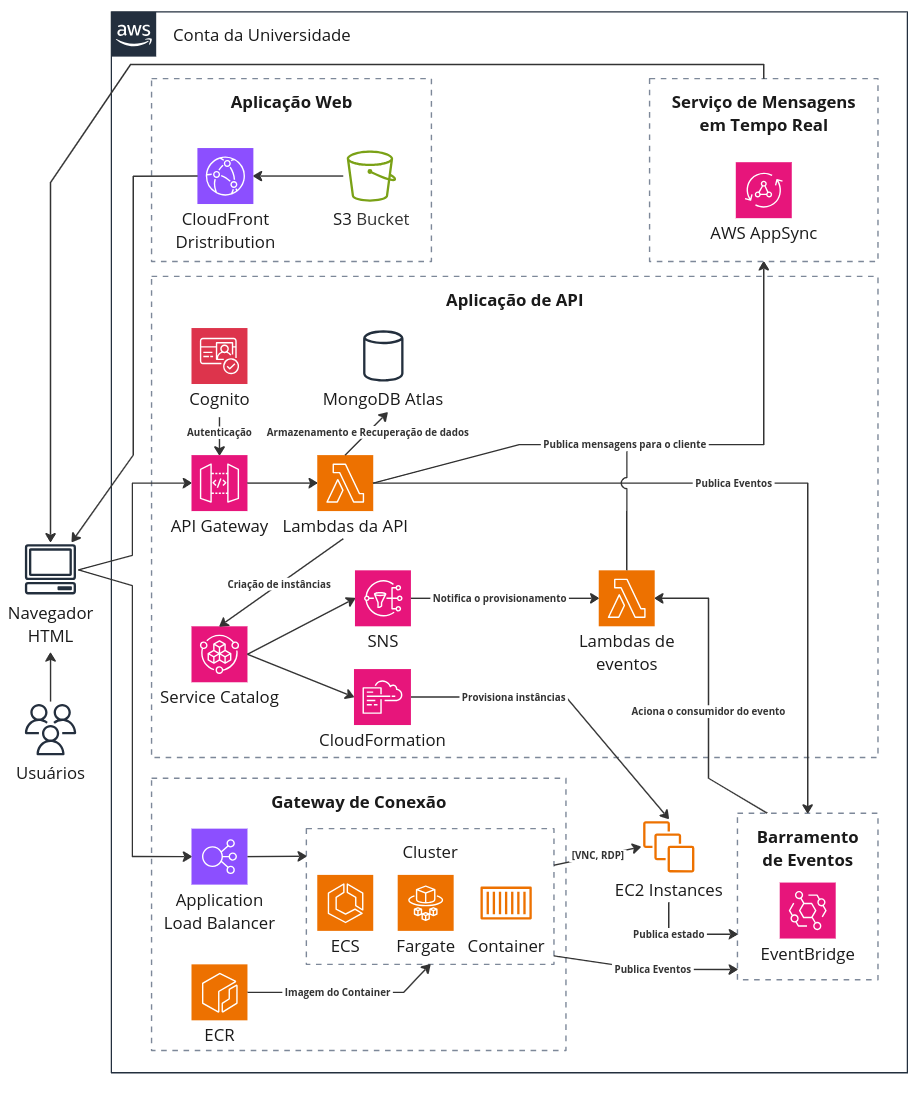
\includegraphics[width=\textwidth]{capitulos/2-metodologia/files/infra-diagram.png}
\fonte{Autoria Própria (2024)}
\end{figure}

A implantação do \textit{Virtual Lab} depende do acesso a uma conta da \gls{aws} com permissões administrativas para criar e gerenciar todos os serviços descritos na \autoref{sec:ferramentasETecnologias}. 

Além disso, é necessário ter o utilitário de linha de comando \textit{aws-cli} instalado e configurado com as credenciais de acesso configuradas, visto que o processo é automatizado. \citep{awsclidocs}. A documentação mais detalhada sobre o processo de configuração do \textit{aws-cli} pode ser encontrada no site oficial da \gls{aws}, bem como na documentação do repositorio do projeto.

A seguir são descritas as etapas necessárias para a implantação a partir do código fonte do sistema, utilizando um computador com as seguintes configurações:

\begin{itemize}
    \item Sistema operacional: \textit{Ubuntu 24.04 LTS}
    \item Processador: \textit{Intel Core i7-1165G7 CPU @ 2.80GHz x 8}
    \item Memória \gls{ram}: 15,3 GiB 
    \item Espaço em disco: 472,8 GiB
\end{itemize}

Contando também com os seguintes softwares instalados:

\begin{itemize}
    \item \textit{Node.js} versão 18.19.0
    \item \textit{npm} versão 10.2.3
    \item \textit{Docker} versão 24.0.5
    \item \textit{aws-cli} versão 2.11.9
\end{itemize}

\subsection{Configuração das dependências}
\label{subsec:configuracaoDasDependencias}

Com o código fonte do sistema em mãos, o primeiro passo é instalarm todas as dependências do projeto. Para isso, basta executar o seguinte comando em um terminal na raiz do projeto:

\shellcmd{npm install}

Esse comando irá instalar todas as dependências do projeto, incluindo as dependências de desenvolvimento, que também são necessárias para o processo de implantação.

Com o término da execução, uma nova pasta chamada \textit{node\_modules} será criada na raiz do projeto, contendo todas as dependências instaladas.

\subsection{Variáveis de ambiente}
\label{subsec:variaveisDeAmbienteEFeatureFlags}

O próximo passo é configurar as variáveis de ambiente do sistema. Elas são necessárias para a identificação das credenciais de acesso à \gls{aws}, bem como para a configuração do comportamento de certos componentes do sistema.

A primeira etapa é criar um novo arquivo chamado \textit{.env} na raiz do projeto. No projeto existe um arquivo chamado \textit{.env.example} que contém um exemplo das variáveis de ambiente necessárias. Para criar uma cópia desse arquivo, basta executar o seguinte comando:

\shellcmd{cp .env.example .env}

Todas variáveis do arquivo são opcionais, por se tratarem de variáveis de ambiente, o sistema irá utilizar valores padrão caso as variáveis não sejam definidas. A seguir é apresentada uma lista das variáveis de ambiente disponíveis e suas descrições:

\begin{itemize}
    \item \textit{READABLE\_LOG\_FORMAT}: Define o formato dos logs do sistema. Quando definido como \textit{true}, os logs serão formatados de forma legível. Caso contrário, os logs serão formatados de forma compacta. O valor padrão é \textit{false}.

    \item \textit{RETAIN\_USER\_POOL\_ON\_DELETE}: Define se o \textit{AWS Cognito User Pool} deve ser mantido após a exclusão do sistema. Quando definido como \textit{true}, o \textit{User Pool} será mantido. Caso contrário, o \textit{User Pool} será excluído. O valor padrão é \textit{false}. Em ambientes de produção, é recomendado manter o \textit{User Pool} após a exclusão do sistema, para que os usuários possam ser recuperados em caso de falha.

    \item \textit{USER\_POOL\_IDENTITY\_PROVIDER}: Define se um provedor de identidade externo deve ser utilizado em conjunto com o \textit{AWS Cognito User Pool}. Quando definido como \textit{true}, um provedor de identidade externo será utilizado e um botão será habilitado na tela de \textit{login} para utilizar essa funcionalidade. Caso contrário, o provedor de identidade padrão da \gls{aws} será utilizado. O valor padrão é \textit{false}. Caso essa variável seja definida como \textit{true}, as seguintes variáveis de ambiente também deverão ser definidas:

    \begin{itemize}
        \item \textit{USER\_POOL\_IDENTITY\_PROVIDER\_CLIENT\_ID}: O ID do cliente do provedor de identidade externo.

        \item \textit{USER\_POOL\_IDENTITY\_PROVIDER\_CLIENT\_SECRET}: O segredo do cliente do provedor de identidade externo.

        \item \textit{USER\_POOL\_IDENTITY\_PROVIDER\_ISSUER\_URL}: A URL do provedor de identidade externo.
    \end{itemize}

    \item \textit{USER\_POOL\_SELF\_SIGN\_UP}: Define se os usuários podem se cadastrar no sistema por conta própria. Quando definido como \textit{true}, o auto-cadastro será permitido e o cliente web apresentará uma tela de cadastro. Caso contrário, o auto-cadastro será desativado e o cliente web esconderá a tela de cadastro. O valor padrão é \textit{false}. Vale lembrar que usuários auto-cadastrados recebem uma permissão de usuário pendente e precisam ser aprovados por um administrador antes de poderem acessar o sistema.

    \item \textit{NEW\_RELIC\_LAMBDA\_INSTRUMENTATION}: Define se a instrumentação do \textit{New Relic} deve ser ativada para as funções \textit{Lambda}. Quando definido como \textit{true}, a instrumentação será ativada. Caso contrário, a instrumentação será desativada. O valor padrão é \textit{false}. Caso essa variável seja definida como \textit{true}, as seguintes variáveis de ambiente também deverão ser definidas:

    \begin{itemize}

        \item \textit{NEW\_RELIC\_ACCOUNT\_ID}: O ID da conta do \textit{New Relic}.

        \item \textit{NEW\_RELIC\_TRUSTED\_ACCOUNT\_KEY}: Caso a conta do \textit{New Relic} seja gerenciada por outra conta do \textit{New Relic}, o ID da conta gerenciadora, caso contrário, o valor deve ser o mesmo que o \textit{NEW\_RELIC\_ACCOUNT\_ID}.

        \item \textit{NEW\_RELIC\_LICENSE\_KEY}: A chave de licença do \textit{New Relic}.

    \end{itemize}

    \item \textit{CLIENT\_CUSTOM\_DOMAIN}: Define se o cliente web deve ser servido em um domínio personalizado. Quando definido como \textit{true}, o cliente web será servido em um domínio personalizado. Caso contrário, o cliente web será servido em um domínio padrão. O valor padrão é \textit{false}. Caso essa variável seja definida como \textit{true}, as seguintes variáveis de ambiente também deverão ser definidas:

    \begin{itemize}

        \item \textit{CLIENT\_CUSTOM\_DOMAIN\_NAME}: O nome do domínio personalizado. Exemplo: \textit{virtual-lab.example.com}.

        \item \textit{CLIENT\_CUSTOM\_DOMAIN\_CERTIFICATE\_ARN}: O ARN do certificado do domínio personalizado criado manualmente no \textit{AWS Certificate Manager} \citep{awscertificatemanagerdocs}. Essa é o unico recurso que deve ser criado manualmente.

    \end{itemize}

    \item \textit{DOCS\_CUSTOM\_DOMAIN}: Define se o site de documentação deve ser servido em um domínio personalizado. Quando definido como \textit{true}, o site de documentação será servido em um domínio personalizado. Caso contrário, o site de documentação será servido em um domínio padrão. O valor padrão é \textit{false}. Caso essa variável seja definida como \textit{true}, as seguintes variáveis de ambiente também deverão ser definidas:

    \begin{itemize}

        \item \textit{DOCS\_CUSTOM\_DOMAIN\_NAME}: O nome do domínio personalizado. Exemplo: \textit{docs.virtual-lab.example.com}.

        \item \textit{DOCS\_CUSTOM\_DOMAIN\_CERTIFICATE\_ARN}: O ARN do certificado do domínio personalizado criado manualmente no \textit{AWS Certificate Manager} \citep{awscertificatemanagerdocs}. Caso o certificado utilizado no cliente web também suporte o domínio da documentação, essa variável pode receber o mesmo valor da variável \textit{CLIENT\_CUSTOM\_DOMAIN\_CERTIFICATE\_ARN}.

    \end{itemize}

\end{itemize}

Uma forma de indicar quais credenciais de acesso à \gls{aws} o sistema deve utilizar para fazer a implantação é inserir as seguintes variáveis de ambiente no arquivo \textit{.env}:

\begin{itemize}
    \item \textit{AWS\_ACCESS\_KEY\_ID}: O ID da chave de acesso da \gls{aws}.
    \item \textit{AWS\_SECRET\_ACCESS\_KEY}: A chave de acesso secreta da \gls{aws}.
\end{itemize}

\subsection{Comando de implanta\c{c}\~ao}
\label{subsec:comandoDeImplantacao}

Nesse ponto, todos os pré-requisitos foram atendidos e o sistema está pronto para ser implantado. Para isso, basta executar o seguinte comando na raiz do projeto, substituindo \textit{<stage>} por um nome de ambiente desejado (por exemplo, \textit{production} ou \textit{staging}):

\shellcmd{npm run deploy -- --stage <stage>}

Esse comando irá provisionar todos os componentes de infraestrutura necessários na \gls{aws}, bem como implantar os serviços de backend, o cliente web e o site da documentação. O processo pode levar alguns minutos na primeira execução, já que tudo será criado do zero.

Com o processo concluído, uma mensagem de conclusão será exibida no terminal, contendo as URLs de acesso ao cliente web e ao site de documentação. O sistema estará disponível para ser acessado pelos usuários finais.

Caso uma mudança tenha sido feita no código fonte do sistema e seja necessário atualizar a implantação, basta executar o comando de implantação novamente. Apenas os componentes afetados pela mudança serão atualizados, o que torna o processo mais rápido.
